\subsection{绝对正则代数或绝对正规代数}

定义 1.--- 设 \(k\) 为域，\(A\) 为 \(k\)-代数。称 \(A\) 是绝对正则的（相应地绝对正规的）\(^{1}\)，如果环 \(\mathrm{A}_{(k')}\) 对每个有限次纯不可分扩张 \(k'\)（在 \(k\) 上）都是正则的（相应地正规的）。

每个绝对正则（相应地绝对正规）的 \(k\)-代数都是正则的（相应地正规的），在定义 1 中取 \(k' = k\) 即可看出。回忆：\(k\)-代数 A 若使环 \(\mathrm{A}_{(k')}\) 对每个有限次纯不可分扩张 \(k'\)（在 \(k\) 上）都为约化，则它就是 \(k\)-可分代数 (A, V, 第 117 页, 定理 2)。

例.--- 1) 若 k 是完全域，则每个正则（相应地正规）的 k-代数都是绝对正则的（相应地绝对正规的）。

\begin{enumerate}
\def\labelenumi{\arabic{enumi})}
\setcounter{enumi}{1}
\tightlist
\item
  设 A 为 Artin \(k\)-代数。若 A 正规，则它约化，从而同构于 \(k\) 的一些扩张的有限积 (A, VIII, § 8, 第 1 节, 命题 2)。下列条件等价：
\end{enumerate}

A 是可分的；

A 是绝对正则的；

A 是绝对正规的。

事实上，若 A 绝对正规，则它可分；若 A 可分，则对每个有限次纯不可分扩张 \(k'\)（在 \(k\) 上），环 \(\mathrm{A}_{(k')}\) 都是约化的且 Artin 的，从而同构于一些域的积，因而是正则的，于是 \(A\) 是绝对正则的。

此外，若 k-代数 A 是有限次的，则上述条件等价于说 A 是平展的 (A, V, 第 34 页, 定理 4)。

\begin{enumerate}
\def\labelenumi{\arabic{enumi})}
\setcounter{enumi}{2}
\tightlist
\item
  设 A 为正则局部 \(k\)-代数。若扩张 \(\kappa_{\mathrm{A}}\)（在 \(k\) 上）可分，则代数 A 绝对正则。事实上，设 \(k'\) 为 \(k\) 的一个有限扩张。A-模 \(\mathrm{A}_{(k')}\) 是自由的。由于它是有限型的，\(\mathrm{A}_{(k')}\) 的每个极大理想都位于 \(\mathfrak{m}_{\mathrm{A}}\) 之上 (V, § 2, 第 1 节, 命题 1)。环 \(\kappa_{\mathrm{A}} \otimes_{\mathrm{A}} \mathrm{A}_{(k')}\) 同构于 \(\kappa_{\mathrm{A}} \otimes_{k} k'\)，是正则的 (第 3 节, 引理 2)。由 § 4 第 5 节命题 9 的推论，环 \(\mathrm{A}_{(k')}\) 正则，这就证明了 \(k\)-代数 A 绝对正则。
\end{enumerate}

命题 6. 设 k 为域，A 为 Noether k-代数。

\begin{enumerate}
\def\labelenumi{\alph{enumi})}
\item
  若 A 绝对正则（相应地绝对正规、可分），则对 A 的每个乘性子集 S，\(S^{-1}A\) 亦然。
\item
  若对 A 的每个极大理想 m，\(A_{m}\) 都绝对正则（相应地绝对正规、可分），则 A 绝对正则（相应地绝对正规、可分）。
\item
  这由下述事实得出：环 \((\mathrm{S}^{-1}\mathrm{A})_{(k^{\prime})}\) 同构于环 \(\mathrm{A}_{(k^{\prime})}\) 的一个分式环，这对 k 的每个扩张 \(k^{\prime}\) 都成立。
\item
  设对 A 的每个极大理想 m，\(A_{m}\) 都绝对正则（相应地绝对正规、可分）。设 \(k'\) 为 k 的一个有限次纯不可分扩张，设 \(m'\) 为 \(\mathrm{A}_{(k')}\) 的一个极大理想。尚需验证局部环 \((\mathrm{A}_{(k')})_{\mathfrak{m}'}\) 是正则的（相应地正规的、约化的）。
\end{enumerate}

典范同态 \(A \to A_{(k')}\) 使 \(A_{(k')}\) 成为有限 A-代数。理想 \(m'\) 位于 A 的某个极大理想 m 之上 (V, § 2, 第 1 节, 命题 1)，而 \((\mathrm{A}_{(k')})_{\mathfrak{m}'}\) 同构于正则（相应地正规、约化）环 \((\mathrm{A}_{\mathfrak{m}})_{(k')}\) 的一个分式环，因而是正则的（相应地正规的、约化的）。

引理 3.--- 设 k 为域，K 为 k 的一个有限生成扩张。存在 K 的一个有限次扩张 L，以及 L 在 k 上的一个中间扩张 k′，它对 k 是纯不可分的且有限次，使得 L 在 k′ 上的扩张可分。

取定 K 与一个完全闭包 \(\hat{k}\)（在 \(k\) 上）的复合扩张 E，以及 E 的元素组 \((t_1, \ldots, t_n)\)，使得 E 是 \(\hat{k}(t_1, \ldots, t_n)\) 的可分代数扩张。设 I 为 K 在 \(k\) 上的一个有限生成系。域 \(\hat{k}(t_1, \ldots, t_n)\)（相应地 \(\hat{k}\mathrm{K}\)）是子域 \(k'(t_1, \ldots, t_n)\)（相应地 \(k'\mathrm{K}\)）的并，其中 \(k'\) 取遍 \(\hat{k}\) 的对 \(k\) 有限的中间扩张；因此可以找到这样一个中间扩张 \(k'\)，使得元素 \(t_1, \ldots, t_n\)（它们属于 \(\mathrm{E} = \hat{k}\mathrm{K}\)）含于 \(k'\mathrm{K}\)，且 I 的每个元素在 \(k'(t_1, \ldots, t_n)\) 上都是代数的且可分的。于是 \(\mathrm{L} = k'\mathrm{K}\) 是 \(k'\) 的可分扩张且对 K 有限次，而 \(k'\) 是 \(k\) 的有限次纯不可分扩张。

命题 7. 设 \(k\) 为域，A 与 B 为 \(k\)-代数，其中一个是本质有限型的。设 A 绝对正则（相应地绝对正规）。若环 B 正则（相应地正规），则环 A \(\otimes_{k}\) B 亦然。

设 K 为 k 的有限生成扩张；我们来证明环 \(\mathrm{A}_{(\mathrm{K})}\) 正则（相应地正规）。事实上，考察具有引理 3 中性质的扩张 L 与 \(k'\)。于是环 \(\mathrm{A}_{(k')}\) 依定义正则（相应地正规），而环 \(\mathrm{A}_{(\mathrm{L})}\)——它与 \(\mathrm{A}_{(k')} \otimes_{k'} \mathrm{L}\) 恒同——由第 3 节命题 5, b) 是正则的（相应地正规的）。于是由第 3 节命题 5, a)，\(\mathrm{A}_{(\mathrm{K})}\) 正则（相应地正规）。

设环 B 正则（相应地正规），我们来证明命题。典范同态 \(B \to A \otimes_{k} B\) 使 \(A \otimes_{k} B\) 成为自由 B-模。对 B 的每个素理想 p，环 \((A \otimes_{k} B) \otimes_{B} \kappa(\mathfrak{p})\) 由 § 4 第 5 节命题 9 的推论（相应地 § 1 第 10 节定理 4 的推论 3）与 \(A \otimes_{k} \kappa(\mathfrak{p})\) 恒同；我们只需证明对 B 的每个素理想 p，\(A \otimes_{k} \kappa(\mathfrak{p})\) 都正则（相应地正规）。

若 \(k\)-代数 B 本质有限型，则 \(\kappa(\mathfrak{p})\) 在 \(k\) 上的扩张是有限型的，且由上文所见，环 A \(\otimes_k \kappa(\mathfrak{p})\) 正则（相应地正规）。今设 \(k\)-代数 A 本质有限型；环 A \(\otimes_k \kappa(\mathfrak{p})\) 是 Noether 的，并且是 Noether 子环 \(A \otimes_k K\) 的递增有向族之并，其中 \(K\) 取遍 \(\kappa(\mathfrak{p})\) 的有限生成中间扩张。后述这些环都正则（相应地正规），于是可应用第 3 节的引理 1。

推论 1. 设 k 为域。两个绝对正则（相应地绝对正规）的 k-代数（其中一个是本质有限型的）的张量积是绝对正则（相应地绝对正规）的 k-代数。

设 A 与 B 为满足推论假设的两个 k-代数。设 \(k'\) 为 k 的一个有限次纯不可分扩张。环 \(\mathrm{B}_{(k')}\) 正则（相应地正规）；由命题 7，环 \(A \otimes_{k} B_{(k')}\) 正则（相应地正规），而与之同构的环 \((\mathrm{A} \otimes_{k} \mathrm{B}) \otimes_{k} k'\) 亦然。

推论 2.--- 设 k 为域，A 为绝对正则（相应地绝对正规）的 k-代数，K 为 k 的扩张。设 A 本质有限型，或 k 的扩张 K 有限型。

\begin{enumerate}
\def\labelenumi{\alph{enumi})}
\item
  环 \(\mathrm{A}_{(K)}\) 正则（相应地正规）。
\item
  若 k 的扩张 K 可分，则 k-代数 \(\mathrm{A}_{(\mathrm{K})}\) 绝对正则（相应地绝对正规）。
\end{enumerate}

断言 (a) 由命题 7 得出；断言 (b) 由推论 1 与例 2 得出。

推论 3. 设 \(k\) 为域，A 为 \(k\)-代数，K 为 \(k\) 的扩张。设 \(k\)-代数 A 本质有限型，或 \(k\) 的扩张 K 有限型。为使 \(k\)-代数 A 绝对正则（相应地绝对正规），必须且只需 K-代数 \(\mathrm{A}_{(\mathrm{K})}\) 绝对正则（相应地绝对正规）。

设 A 绝对正则（相应地绝对正规），并设 \(K'\) 为 K 的一个有限次纯不可分扩张。环 \(K'\otimes_{K}A_{(K)}\) 同构于 \(K'\otimes_{k}A\)，由推论 2 是正则的（相应地正规的）。

反之，设 K-代数 \(\mathrm{A}_{(\mathrm{K})}\) 绝对正则（相应地绝对正规），并设 \(k'\) 为 \(k\) 的一个有限次纯不可分扩张。设 L 为 \(k'\) 与 K 的一个复合扩张；于是环 \(\mathrm{A}_{(\mathrm{L})}\) 与 \(\mathrm{L} \otimes_{\mathrm{K}} \mathrm{A}_{(\mathrm{K})}\) 恒同，因而是正则的（相应地正规的）；从而由第 3 节命题 5, a)，环 \(\mathrm{A}_{(k')}\) 正则（相应地正规）。

推论 4.--- 设 k 为域，A 为本质有限型的 k-代数，K 为 k 的一个作为完全域的扩张。为使 A 绝对正则（相应地绝对正规），必须且只需环 \(\mathrm{A}_{(\mathrm{K})}\) 正则（相应地正规）。

这由推论 3 与例 1 得出。

\subsection{绝对正则代数的刻画}

命题 8. 设 \(k\) 为域，A 为本质有限型 \(k\)-代数。以 I 表示 \(k\)-代数同态 \(\mu: A \otimes_k A \to A\)（满足 \(\mu(x \otimes y) = xy\)，对 A 中的 \(x\) 与 \(y\)）的核。下列条件等价：

\begin{enumerate}
\def\labelenumi{(\roman{enumi})}
\item
  k-代数 A 绝对正则；
\item
  对每个正则 k-代数 C，环 A ⊗k C 正则；
\item
  环 A ⊗k A 正则；
\item
  A ⊗k A 的理想 I 是完全割的 (§ 5, 第 1 节, 定义 1)。
\end{enumerate}

以 B 表示环 A \(\otimes_{k}\) A，并赋予它由同态 \(\rho: \mathrm{A} \to \mathrm{A} \otimes_{k} \mathrm{A}\)（其中 \(\rho(x) = x \otimes 1\)）导出的 A-代数结构；于是 \(\mu\) 是 A-代数同态，并且通过过渡到商，诱导出从 B/I 到 A 上的同构。

(i)⇒(ii)：由命题 7 得出。

(ii)⇒(iii)：只需对 C=k 再对 C=A 应用 (ii)。

(iii)⇒(iv)：A-模 B 是自由的，从而忠实平坦。若环 B 正则，则 A 正则 (§ 4, 第 5 节, 命题 8)；于是理想 I 是完全割的 (§ 5, 第 3 节, 命题 2)。

(iv)⇒(i)：设理想 I 是完全割的，先证明 A 正则。设 m 为 A 的极大理想，设 \(\nu:(\mathrm{A}/\mathfrak{m})\otimes_{k}\mathrm{A}\to\mathrm{A}/\mathfrak{m}\) 为由 \(\mu\) 导出的同态。极大理想 n=Ker \(\nu\) 等于 \(I((\mathrm{A}/\mathfrak{m})\otimes_{k}A)\)；把 § 5 第 6 节的命题 6 应用于 A-代数 \(A'=A/\mathfrak m\)，可见理想 n 在 \((A/\mathfrak{m})\otimes_{k}A\) 中是完全割的。于是 (§ 5, 第 3 节, 命题 3)，局部环 \(((\mathrm{A}/\mathfrak{m})\otimes_{k}A)_{n}\) 正则。以 \(j:\mathrm{A}\to(\mathrm{A}/\mathfrak{m})\otimes_{k}\mathrm{A}\) 表示同态 \(x\mapsto1\otimes x\)；由于 \(\nu\circ j\) 是从 A 到 A/m 的典范同态，有 \(j^{-1}(\mathfrak{n})=\mathfrak{m}\)。于是 j 延拓为从 \(A_{m}\) 到 \(((\mathrm{A}/\mathfrak{m})\otimes_{k}\mathrm{A})_{n}\) 的局部环的局部同态，这使后者成为忠实平坦的 \(A_{m}\)-模。由 § 4 第 5 节的命题 8，环 \(A_{m}\) 因此正则。我们至此证明了 A 正则。

现在设 \(k'\) 为 \(k\) 的扩张。映射 \(\mu': A_{(k')} \otimes_{k'} A_{(k')} \to A_{(k')}\)（由 \(A_{(k')}\) 的乘法导出）的核正是 \(IA_{(k')}\)；因此它在 \(A_{(k')}\) 中是完全割的 (§ 5, 第 6 节, 命题 6)。于是 \(k'\)-代数 \(A_{(k')}\) 满足条件 (iv)；由刚才所见，它正则，这就证明了 (i)。

回忆 (A, III, 第 133–134 页)：商 I/I² 赋予由 ρ 诱导的 A-模结构后，记作 Ωₖ(A)，称为 A 的 k-微分模。当 k-代数 A 本质有限型时，环 A ⊗ₖ A 是 Noether 的，于是 A-模 Ωₖ(A) 有限生成。

以 \(d_{A/k}\) 或简称 \(d\) 表示一个 \(k\)-线性映射（自 A 到 \(\Omega_k(A)\)），它把 A 的元素 \(x\) 对应为 \(x \otimes 1 - 1 \otimes x\) 在 \(\Omega_k(A)\) 中的类。映射 \(d\) 是 \(k\)-导子；对每个 A-模 M 与每个 \(k\)-导子 D: A → M，存在唯一的 A-线性映射 \(g: \Omega_k(A) \to M\) 使 D = g ∘ d (同上引文, 命题 18)。

若 S 是 A 的乘性子集，则典范 \(S^{-1}A\)-线性映射 (同上引文, 第 136 页)

\[
\mathrm{S} ^ {- 1} \Omega_ {k} (\mathrm{A}) \rightarrow \Omega_ {k} (\mathrm{S} ^ {- 1} \mathrm{A})
\]

是双射的：事实上，只需验证：对每个 S \(^{-1}\) A-模 M，每个 k-导子 D : A → M 都唯一扩张为 k-导子 D : S \(^{-1}\) A → M；这由同上引文第 123 页命题 5 的论证得出。

设 \(k\) 为域，A 为本质有限型局部 \(k\)-代数。令 \(n = \dim(A) + \deg.\mathrm{tr}_k(\kappa_A)\)。设 B 为有限生成 \(k\)-代数，\(\mathfrak{q}\) 为 B 的素理想，使 \(k\)-代数 A 同构于 \(\mathbf{B}_{\mathfrak{q}}\)（\(cf.\ n^{\circ} 1\)，例 2）；我们有 \(n = \dim_{\mathfrak{q}}(\mathbf{B})\) (VIII, § 2, 第 4 节, 定理 3 的推论 5)。由同上引文定理 3, c) 与推论 5，还有

\[
n = \sup \deg . \operatorname{tr} _ {k} (\kappa (\mathfrak {p}))
\]

其中 p 取遍 A 的极小素理想的有限族。若 A 是整的，则 n 就是 A 的分式域的超越次数。

定理 1. 设 \(k\) 为域，A 为本质有限型局部 \(k\)-代数。令 \(n = \dim(A) + \deg.\mathrm{tr}_{k}(\kappa_{A})\)。

\begin{enumerate}
\def\labelenumi{\alph{enumi})}
\item
  有 \([\kappa_{A} \otimes_{A} \Omega_k(A): \kappa_{A}] \geqslant n\)。
\item
  下列条件等价：
\end{enumerate}

\begin{enumerate}
\def\labelenumi{(\roman{enumi})}
\item
  k-代数 A 绝对正则；
\item
  A-模 \(\Omega_{k}(\mathrm{A})\) 是秩为 \(n\) 的自由模；
\end{enumerate}

\[
\left[ \kappa_ {A} \otimes_ {A} \Omega_ {k} (A): \kappa_ {A} \right] = n
\]

考察断言

(iii′) 有 \([\kappa_{\mathrm{A}} \otimes_{A} \Omega_k(\mathrm{A}):\kappa_{\mathrm{A}}] \leqslant n\)；

显然 (ii) 蕴含 (iii)，且 (iii) 蕴含 (iii′)。为证明定理，只需证明蕴含关系 (i) \(\Rightarrow\) (ii) 与 (iii′) \(\Rightarrow\) (i)。

选取有限生成 \(k\)-代数 B 及 B 的素理想 \(\mathfrak{q}\)，使 A 同构于 \(\mathrm{B}_{\mathfrak{q}}\) (\(n^{\circ} 1\), 例 2)。我们有 \(\dim_{\mathfrak{q}}(\mathrm{B}) = n\)；把 B 换成环 \(\mathrm{B}_f\)（其中 \(f \in \mathrm{B} - \mathfrak{q}\)），可以要求 B 的谱连通且维数为 \(n\)，以下即作此假设。

\begin{enumerate}
\def\labelenumi{(\roman{enumi})}
\tightlist
\item
  \(\Rightarrow\) (ii)：设 \(k\)-代数 A 绝对正则。如同命题 8 的证明，以 \(\mu : A \otimes_k A \to A\) 与 \(\nu : \kappa_A \otimes_k A \to \kappa_A\) 表示由 A 的乘法导出的同态；令 I = \(\operatorname{Ker}(\mu)\)，\(\mathfrak{n} = \operatorname{Ker}(\nu)\)。理想 I 是完全割的；理想 \(\mathfrak{n}\) 极大，且局部环 (\(\kappa_A \otimes_k A\) ) \(_{\mathfrak{n}}\) 正则 (同上引文)。由 § 5 第 2 节的定理 1，有限型 \(A\)-模 I/I²——它正是 \(\Omega_k(A)\)——是投射的，从而是自由的。但依 § 5 第 6 节的注，理想 \(\mathfrak{n}\) 与 \(\kappa_A \otimes_A 1\) 恒同，于是 \(\mathfrak{n}/\mathfrak{n}^2\) 同构于 \(\kappa_A \otimes_A \Omega_k(A)\)。因此有
\end{enumerate}

\[
\operatorname{rg} \left(\Omega_ {k} (\mathrm{A})\right) = \left[ \kappa_ {\mathrm{A}} \otimes_ {k} \Omega_ {k} (\mathrm{A}): \kappa_ {\mathrm{A}} \right] = \left[ \mathfrak {n} / \mathfrak {n} ^ {2}: \kappa_ {\mathrm{A}} \right] = \dim \left(\kappa_ {\mathrm{A}} \otimes_ {k} \mathrm{A}\right) _ {\mathfrak {n}}.
\]

以 B′ 表示环 \(\kappa_{A}\otimes_{k}B\)，以 S 表示 B-q 在 B′ 中的像。环 \(\kappa_{A}\otimes_{k}A\) 与 B′ \(\otimes_{B}B_{q}\) 恒同，亦即与 S \(^{-1}\) B′ 恒同。因此存在一个不与 S 相交的极大理想 \(q'\)（属于 \(B'\)），使得 \(n = S^{-1}q'\) 成立；于是环 \((\kappa_A \otimes_k A)_n\) 同构于 \(B_{q'}'\)，且有

\[
\dim (\kappa_ {A} \otimes_ {k} A) _ {\mathfrak {n}} = \dim (\kappa_ {A} \otimes_ {k} B) _ {\mathfrak {q} ^ {\prime}} = \dim_ {\mathfrak {q} ^ {\prime}} (\kappa_ {A} \otimes_ {k} B).
\]

由于 n 包含 \(\kappa_{\mathrm{A}} \otimes_{k} qB_{q}\)，\(q'\) 包含理想 \(\kappa_{\mathrm{A}} \otimes q\)（\(B'\) 中的），于是它在 B 中的逆像包含 \(q\)；该逆像等于 \(q\)，因为 \(q'\) 不与 S 相交。由 VIII, § 2, 第 4 节, 命题 5 的推论，有

\[
\dim_ {\mathfrak {q} ^ {\prime}} \left(\kappa_ {A} \otimes_ {k} B\right) = \dim_ {\mathfrak {q}} (B) = n,
\]

这就证明了 (ii)。

(iii′) \(\Rightarrow\) (i)：设 \([\kappa_{\mathrm{A}}\otimes_{\mathrm{A}}\Omega_{k}(A):\kappa_{\mathrm{A}}]\leqslant n\)，即 \([\kappa (\mathfrak{q})\otimes_{\mathrm{B}}\Omega_{k}(\mathrm{B}):\kappa (\mathfrak{q})]\leqslant n\)，我们来证明 \(k\)-代数 B 绝对正则。设 \((x_{1},\ldots ,x_{n})\) 为 B 的元素序列，使 \(1\otimes dx_1,\dots ,1\otimes dx_n\) 生成 \(\kappa (\mathfrak{q})\)-向量空间 \(\kappa (\mathfrak{q})\otimes_{\mathrm{B}}\Omega_{k}(\mathrm{B})\)。把 B 换成 \(\mathrm{B}_f\)（\(f\) 为 \(\mathrm{B} - \mathfrak{q}\) 中适当选取的元素），可设 \(dx_{1},\ldots ,dx_{n}\) 生成 B-模 \(\Omega_k(\mathrm{B})\)。由 Nakayama 引理与 II, § 5, 第 1 节, 命题 2，设 \(\bar{k}\) 为 \(k\) 的代数闭扩张。我们只需证明 \(\bar{k}\)-代数 \(\mathrm{B}_{(\bar{k})}\) 正则，因为这将蕴含 B 绝对正则 (第 4 节命题 7 的推论 4)。对 \(\mathrm{B}_{(k)}\) 的每个典范分支 C，微分 \(d(1\otimes x_i)\) 生成 C-模 \(\Omega_{\bar{k}}(\mathrm{C})\) (A, III, § 10, 第 12 节, 命题 20)。于是定理由下面两个引理得出：

引理 4.—设 \(k\) 为域，K 为 \(k\) 的代数扩张。设 B 为谱连通的 \(k\)-代数。对 \(\mathrm{B}_{(\mathrm{K})}\) 的每个典范分支 C，有 \(\dim(\mathrm{C}) = \dim(\mathrm{B})\)。

先处理扩张 K 对 \(k\) 有限的情形。B-模 C 是自由模的直和项，从而是有限生成投射模。由于函数 \(\mathfrak{p} \mapsto \mathrm{rg}_{\mathfrak{p}}\) 在 \(\operatorname{Spec}(B)\) 上取常值 (II, § 5, 第 3 节)，B-模 C 的支撑集等于 \(\operatorname{Spec}(B)\)，于是 B-模 C 忠实平坦。这蕴含 \(\dim(C) \geqslant \dim(B)\) (VIII, § 2, 第 1 节, 命题 2)，从而得到所欲的等式，因为有 \(\dim(C) \leqslant \dim(B_{(K)}) = \dim(B)\) (VIII, § 2, 第 4 节, 命题 5 的推论)。

对一般情形，设 \(e\) 为 \(B_{(K)}\) 的幂等元，使 \(C = B_{(K)}/B_{(K)}e\)。存在一个有限次中间扩张 \(K'\)（在 \(K\) 上），使 \(e\) 是某个幂等元 \(e'\)（它属于 \(B_{(K')}\)）的像。令 \(C' = B_{(K')} / B_{(K')}e'\)。环 \(C' \otimes_{K'} K\) 与 \(C\) 恒同，且 \(C'\) 是 \(B_{(K')}\) 的一个典范分支。由已处理的情形有 \(\dim(C') = \dim(B)\)，又由同上引文有 \(\dim(C') = \dim(C)\)，引理得证。

引理 5.—设 \(k\) 为代数闭域，A 为谱连通的有限型 \(k\)-代数，\(n\) 为整数，\((x_{1},\ldots,x_{n})\) 为 A 的元素的一个有限序列。假设 A 的维数为 \(n\)，且微分 \(dx_{1},\ldots,dx_{n}\) 生成 A-模 \(\Omega_{k}(\mathrm{A})\)。则环 A 是整的且正则的，且 \(A\)-模 \(\Omega_{k}(\mathrm{A})\) 是自由的，以 \((dx_{1},\ldots,dx_{n})\) 为基。

设 \(\mathfrak{m}\) 为 A 的极大理想且 \(\dim(A_{\mathfrak{m}})=n\)。有 \([A/\mathfrak{m}:k]=1\) (V, § 3, 第 3 节, 命题 1 (iii))，于是 \(A=\mathfrak{m}\oplus k1_{A}\)。设 \(p\) 与 \(q\) 为相应的射影

对 \(a\) 与 \(b\)（\(A\) 中的元素），有

\[
a b = \left(p (a) q (b) + q (a) p (b) + p (a) p (b), q (a) q (b)\right),
\]

从而 \(p(ab) \equiv p(a)q(b) + q(a)p(b) \pmod{\mathfrak{m}^{2}}\)。于是，映射 \(\delta: A \to \mathfrak{m}/\mathfrak{m}^{2}\)（它把 A 的每个元素 x 对应为 \(p(x)\) 模 \(\mathfrak{m}^{2}\) 的类）是 A 到 k-向量空间 \(\mathfrak{m}/\mathfrak{m}^{2}\) 的 k-导子。因此存在 A-线性映射 \(\phi: \Omega_{k}(A) \to \mathfrak{m}/\mathfrak{m}^{2}\)，使 \(\delta(x) = \phi(dx)\) 对每个 \(x \in A\) 都成立。由于 \(\delta\) 是满射，诸 \(\phi(dx_{i})\) 生成 A/m-向量空间 \(\mathfrak{m}/\mathfrak{m}^{2}\)，且有 \([\mathfrak{m}/\mathfrak{m}^{2}: A/\mathfrak{m}] \leqslant n = \dim(A_{\mathfrak{m}})\)。由此推出 \(A_{\mathfrak{m}}\) 正则，且诸 \(dx_{i}\) 的像构成 A/m-向量空间 A/m \(\otimes_{A} \Omega_{k}(A)\) 的一组基。

现在证明环 A 是整的且正则的。存在 A 的极小素理想 q 使 \(\dim(A/q) = n\)。对 A 的每个包含 q 的极大理想 m，有 \(\dim(A_{\mathfrak{m}}) = n\) (VIII, § 2, 第 4 节, 定理 3 的推论 2)，于是由刚才所见，\(A_{\mathfrak{m}}\) 正则。特别地，\(A_{\mathfrak{m}}\) 是整的，这蕴含 \(qA_{\mathfrak{m}} = 0\)。由于这对 V(q) 的所有极大理想 m 都成立，我们推出 \(\operatorname{Supp}(\mathfrak{q}) \cap V(\mathfrak{q}) = \varnothing\)。但 \(\operatorname{Spec}(A)\) 连通，V(q) 非空，且有 \(\operatorname{Supp}(\mathfrak{q}) \cup V(\mathfrak{q}) = \operatorname{Spec}(A)\) (II, § 4, 第 4 节, 命题 16)。由此推出 \(\operatorname{Supp}(\mathfrak{q}) = \varnothing\)，从而 q = 0，这意味着 A 是整环。于是对 A 的每个极大理想 m 都有 \(\dim(A_{\mathfrak{m}}) = n\)；应用证明的第一部分，推出 A 正则。

最后，设 \(\sum_{i=1}^{n} a_i dx_i = 0\) 为诸 \(dx_i\) 之间的一个系数在 \(A\) 中的线性关系。若诸 \(a_i\) 不全为零，则存在指标 \(i\) 与 A 的极大理想 \(\mathfrak{m}\)，使 \(a_i\) 不属于 \(\mathfrak{m}\) (V, § 3, 第 3 节, 命题 1, (iii) 与 (iv))；但这与上面已证的事实矛盾：诸 \(dx_i\) 在 (A/m) \(\otimes_{\mathrm{A}} \Omega_k(\mathrm{A})\) 中的类线性无关。

例.--- 当 A 是 k 的有限生成扩张时，结合第 4 节的例 2，定理 1 重新给出 A, V, 第 128 页的推论 1。

推论 1. - 设 \(k\) 为域，\(A\) 为本质有限型 \(k\)-代数。素理想 \(\mathfrak{p}\)（属于 \(\operatorname{Spec}(A)\)）中，使 \(k\)-代数 \(\mathrm{A}_{\mathfrak{p}}\) 绝对正则的那些构成 \(\operatorname{Spec}(A)\) 的一个开子集。

可以假设 \(k\)-代数 A 是有限生成的。于是所考虑的集合由这样的素理想 \(\mathfrak{p}\) 组成：\([\kappa(\mathfrak{p}) \otimes_k \Omega_k(A) : \kappa(\mathfrak{p})] \leqslant \dim_{\mathfrak{p}}(A)\)。而函数 \(\mathfrak{p} \mapsto \dim_{\mathfrak{p}}(A)\) 依定义是下半连续的，函数 \(\mathfrak{p} \mapsto [\kappa(\mathfrak{p}) \otimes_k \Omega_k(A) : \kappa(\mathfrak{p})]\) 是上半连续的 (由 Nakayama 引理与 II, § 5, 第 1 节, 命题 2)。

我们稍后将看到 (§ 7, 第 9 节, 定理 3 的推论 4)：在推论 1 的假设下，A 中使环 \(A_{p}\) 正则的素理想 p 组成的集合在 \(\operatorname{Spec}(A)\) 中是开的。

推论 2.--- 设 \(k\) 为域，A 为本质有限生成的 \(k\)-代数。为使 A 绝对正则，必须且只需 A-模 \(\Omega_{k}(A)\) 是投射的，且对 A 的每个极小素理想 \(\mathfrak{q}\)，\(k\)-代数 \(\mathrm{A}_{\mathfrak{q}}\) 都是可分的。

设 A 绝对正则。对 A 的每个素理想 p，k-代数 \(A_{p}\) 绝对正则，于是 \(A_{p}\)-模 \(\Omega_{k}(A_{p})\) 是自由的 (定理 1)；由此推出 A-模 \(\Omega_{k}(A)\) 是投射的 (II, § 5, 第 2 节, 定理 1)。此外，对 A 的每个极小素理想 q，局部 k-代数 \(A_{q}\) 是 Artin 的且绝对正则，从而是一个域，即 k 的可分扩张 (第 4 节, 例 2)。

反之，设 A-模 \(\Omega_{k}(\mathbf{A})\) 是投射的，且 \(k\)-代数 \(\mathbf{A}_{\mathfrak{q}}\) 对每个极小素理想 \(\mathfrak{q}\)（\(\mathbf{A}\) 的）都可分。设 \(\mathfrak{p}\) 为 \(\mathbf{A}\) 的素理想，\(\mathfrak{q}\) 为 \(\mathbf{A}\) 的一个极小素理想（含于 \(\mathfrak{p}\)）。由于 \(\mathbf{A}_{\mathfrak{p}}\)-模 \(\Omega_{k}(\mathbf{A})_{\mathfrak{p}}\) 是自由的 (II, § 3, 第 2 节, 命题 5 的推论 2)，有

\[
[ \kappa (\mathfrak {p}) \otimes_ {\mathrm{A}} \Omega_ {k} (\mathrm{A}): \kappa (\mathfrak {p}) ] = [ \kappa (\mathfrak {q}) \otimes_ {\mathrm{A}} \Omega_ {k} (\mathrm{A}): \kappa (\mathfrak {q}) ].
\]

\(k\)-代数 \(\mathrm{A}_{\mathfrak{q}}\) 是 Artin 的且可分的，从而绝对正则 (\(n^{\circ}\) 4, 例 2)。定理 1 蕴含

\[
[ \kappa (\mathfrak {q}) \otimes_ {\mathrm{A}} \Omega_ {k} (\mathrm{A}): \kappa (\mathfrak {q}) ] = \deg . \operatorname{tr} _ {k} (\kappa (\mathfrak {q})).
\]

于是由定理 1 推出 \(k\)-代数 \(\mathrm{A}_{\mathfrak{p}}\) 绝对正则，推论得证。

注.--- 设 k-代数 A 绝对正则。于是 A 的全分式环 F 与诸 \(A_{q}\) 的积恒同，其中 q 取遍 A 的极小素理想组成的集合 (IV, § 2, 第 5 节, 命题 10)；因此它是可分 k-代数。反之，设 F 是可分 k-代数；对 A 的每个极小素理想 q，k-代数 \(A_{q}\) 是 F 的一个分式环 (IV, § 1, 第 1 节, 命题 2 的推论 3 与第 3 节, 命题 7 的推论 1)，从而是可分 k-代数 (第 4 节, 命题 6)。此外，若 A-模 \(\Omega_{k}(A)\) 是投射的，则由推论 2 推出 k-代数 A 绝对正则。

推论 3.--- 设 \(k\) 为特征 0 的域，A 为本质有限型 \(k\)-代数。为使 A 正则，必须且只需 A-模 \(\Omega_{k}(\mathrm{A})\) 是投射的。

由推论 2，只需证明：若 Artin 局部 \(k\)-代数 A 使 \(\Omega_k(A)\) 为自由 A-模，则 A 是域。而由 IX, § 3, 第 3 节, 定理 1，存在 A 的子域 K 使 \(A = K \oplus \mathfrak{m}_A\)。设 \(\delta: A \to \mathfrak{m}_A / \mathfrak{m}_A^2\) 为 A 到 \(\mathfrak{m}_A\) 上的投影与典范映射 \(\mathfrak{m}_A \to \mathfrak{m}_A / \mathfrak{m}_A^2\) 的复合。如引理 4 的证明那样，可验证 \(\delta\) 是 k-导子。但 A 到某个 A-模的每个 \(k\)-导子都零化 \(\mathfrak{m}_A\)：事实上，设 \(x \in \mathfrak{m}_A\)，选取整数 \(n \geqslant 1\) 使 \(x^{n-1} \neq 0\) 且 \(x^n = 0\)。这在 A-模 \(\Omega_k(A)\) 中蕴含关系 \(nx^{n-1} dx = 0\)，从而 \(dx = 0\)（因为 \(nx^{n-1} \neq 0\)）。于是 \(\delta(\mathfrak{m}_A) = 0\)，从而 \(\mathfrak{m}_A = \mathfrak{m}_A^2\)，最终得 \(\mathfrak{m}_A = \{0\}\)。

\section{光滑代数}

\subsection{导子与同态的提升}

设 \(k\) 为环，C 为 \(k\)-代数，N 为 C 的平方零理想。以 \(\pi : \mathrm{C} \to \mathrm{C/N}\) 表示典范同态；由于 \(\mathrm{N}^2 = \{0\}\)，N 的 C-模结构来自一个 C/N-模结构。

设 A 为 \(k\)-代数，\(\varphi : \mathrm{A} \to \mathrm{C/N}\) 为 \(k\)-代数同态。赋予 N 由 \(\varphi\) 导出的 A-模结构。我们称一个 \(lifting\)（提升；到 C 中）指的是 \(\varphi\) 的任一 \(k\)-代数同态 \(\tilde{\varphi} : \mathrm{A} \to \mathrm{C}\)，它满足 \(\pi \circ \tilde{\varphi} = \varphi\)。设 \(\tilde{\varphi}\) 为这样一个提升，\(\delta\) 为从 A 到 N 中的映射；以 \(\delta + \tilde{\varphi}\) 表示映射 \(x \mapsto \delta(x) + \tilde{\varphi}(x)\)（从 \(A\) 到 C 中）。

命题 1.--- 若 φ 有一个提升，则映射 (δ, φ) ↦ δ + φ 定义了 A 到 N 中的 k-导子群在 φ 的提升集合上的一个单可递作用。

设 \(\tilde{\varphi}_{0}: A \to C\) 为 \(\varphi\) 的一个提升。映射 \(\delta \mapsto \delta + \tilde{\varphi}_{0}\) 诱导出从 \(A\) 到 \(N\) 中的映射的集合到映射 \(\tilde{\varphi}: A \to C\)（满足 \(\pi \circ \tilde{\varphi} = \varphi\)）组成的集合上的一个双射。固定 \(\delta\)，令 \(\tilde{\varphi} = \delta + \tilde{\varphi}_{0}\)。为使 \(\tilde{\varphi}\) 是 \(k\) -代数同态，必须且只需 \(\delta\) 是一个 \(k\)-导子（自 \(A\) 到 \(N\) 中）：事实上，对 \(x, y\)（\(A\) 中的）与 \(\lambda\)（\(k\) 中的），有关系式

\[
\begin{array}{c} \tilde {\varphi} (x + y) - \tilde {\varphi} (x) - \tilde {\varphi} (y) = \delta (x + y) - \delta (x) - \delta (y) \\ \tilde {\varphi} (\lambda x) - \lambda \tilde {\varphi} (x) = \delta (\lambda x) - \lambda \delta (x) \\ \tilde {\varphi} (x y) - \tilde {\varphi} (x) \tilde {\varphi} (y) = \delta (x y) - \delta (x) \delta (y) - \delta (x) \tilde {\varphi} _ {0} (y) - \tilde {\varphi} _ {0} (x) \delta (y) \\ = \delta (x y) - \varphi (x) \delta (y) - \varphi (y) \delta (x), \end{array}
\]

最后一处等式由 N 的平方为零这一事实得出。命题得证。

例.--- 设 B 为 k-代数，N 为 B-模。赋予 k-模 B⊕N 以由 \((b,x)(b',x') = (bb',bx' + b'x)\) 定义的 k-代数结构 (参见 A, III, 第 127 页)，于是 N 是 B ⊕ N 中的平方零理想。设 \(\varphi : A \to B\) 为 k-代数同态。于是 \(\varphi\) 到 B ⊕ N 中的提升恰是形如 \(x \mapsto (\varphi(x), \delta(x))\) 的映射，其中 \(\delta\) 取遍 A 到 N 中的 k-导子的集合 (参见同上引文, 命题 12)。

设 \(\Omega_{k}(A)\) 为环 A 的 \(k\)-微分模，\(d: \mathrm{A} \longrightarrow \Omega_{k}(\mathrm{A})\) 为泛 \(k\)-导子 (A, III, 第 133–134 页)；回忆 (同上引文)：对每个 A-模 M，映射 \(v \mapsto v \circ d\) 是从 \(\mathrm{Hom}_{\mathrm{A}}(\Omega_{k}(A), \mathrm{M})\) 到 A 到 M 中的 \(k\)-导子组成的 A-模上的 A-线性同构。

设 J 为 A 的理想。据 A, III, 第 137 页，有 A/J-线性映射的正合列

\[
\mathrm{J} / \mathrm{J} ^ {2} \stackrel {\bar {d}} {\longrightarrow} (\mathrm{A} / \mathrm{J}) \otimes_ {\mathrm{A}} \Omega_ {k} (\mathrm{A}) \longrightarrow \Omega_ {k} (\mathrm{A} / \mathrm{J}) \rightarrow 0,
\]

其中 \(\bar{d}\) 是由 \(d\) 在 J 上的限制过渡到商而导出的同态。

设 \(\rho : A \to A/J^{2}\) 与 \(\pi : A/J^{2} \to A/J\) 为典范满射。设 \(v : (A/J) \otimes_{A} \Omega_{k}(A) \longrightarrow J/J^{2}\) 为一个 \(k\)-线性映射；对它结合一个 \(k\)-线性映射 \(H_{v} : A \to A/J^{2}\)，令 \(H_{v}(x) = \rho(x) - v(1 \otimes dx)\)。若 \(v\) 是 \(\bar{d}\) 的一个收缩，则 \(H_{v}\) 在 \(J\) 上为零，从而通过过渡到商诱导出 \(k\)-线性映射 \(h_{v} : A/J \to A/J^{2}\)。另一方面，给定 \(k\)-线性映射 \(h : A/J \to A/J^{2}\)，以 \(\psi_{h} : A/J \oplus J/J^{2} \longrightarrow A/J^{2}\) 表示映射 \((x,y) \mapsto h(x)+y\)。

命题 2. - 赋予 \(k\)-模 \(A / J \oplus J / J^2\) 以上面例子中定义的 \(k\)-代数结构。映射 \(v \mapsto h_v\) 与 \(h \mapsto \psi_h\) 诱导出下列集合之间的双射：

\begin{enumerate}
\def\labelenumi{(\roman{enumi})}
\item
  \(\bar{d}\) 的 A/J-线性收缩 v 组成的集合；
\item
  k-代数同态 \(h: A/J \to A/J^{2}\) 中满足 \(\pi \circ h = Id_{A/J}\) 者组成的集合；
\item
  k-代数同构 \(\psi : \mathrm{A} / \mathrm{J} \oplus \mathrm{J} / \mathrm{J}^2 \longrightarrow \mathrm{A} / \mathrm{J}^2\)（满足 \(\pi \circ \psi = \mathrm{pr}_1\) 且 \(\psi(0, z) = z\)，对 \(z \in \mathrm{J} / \mathrm{J}^2\)）组成的集合。
\end{enumerate}

以 \(C = A / J^2\) 与 \(N = J / J^2\) 应用命题 1。设 \(\varphi : A \to A / J\) 为典范满射；同态 \(\rho\) 是 \(\varphi\) 到 \(A / J^2\) 中的一个提升。A-模 \(\text{Hom}_{A / J}((A / J) \otimes_A \Omega_k(A), J / J^2)\) 与 \(\text{Hom}_A(\Omega_k(A), J / J^2)\) 恒同；由命题 1，映射 \(v \mapsto H_v\) 是从这个集合到 \(\varphi\) 到 \(A / J^2\) 中的提升集合上的双射。为证 \(x \in J\) 时有 \(1 \otimes dx = \bar{d}(\rho(x))\)；为使 \(H_v\) 在 \(J\) 上为零，必须且只需 \(v \circ \bar{d}\) 是 \(J / J^2\) 的恒同映射。这就证明了映射 \(v \mapsto h_v\) 在陈述中所述前两个集合之间诱导出双射。

映射 \(h \mapsto \psi_h\) 是从 \(k\)-线性映射（自 A/J 到 A/J \(^2\)）组成的集合，到 \(k\)-线性映射 \(\psi : \text{A/J} \oplus \text{J/J}^2 \longrightarrow \text{A/J}^2\)（满足 \(\psi(0,z) = z\)，对 \(z \in \text{J/J}^2\)）组成的集合上的双射；此外，为使 \(\pi \circ \psi_h = \text{pr}_1\)，必须且只需 \(\pi \circ h = \text{Id}_{\text{A/J}}\)，即有 \(z \equiv h(\pi(z)) \pmod{\text{J/J}^2}\)（对每个 \(z \in \text{A/J}^2\)）。设这些条件满足。为使 \(h\) 是环同态，必须且只需 \(\psi_h\) 亦然；此外，同态 \(\psi_h\) 是双射的：其逆映射把元素 \(z\)（A/J \(^2\) 中的）对应为偶 \((\pi(z), z - h(\pi(z)))\)。这就证明了映射 \(h \mapsto \psi_h\) 在陈述中所述后两个集合之间诱导出双射。

\subsection{形式光滑代数}

设 \(k\) 为环，A 为 \(k\)-线性拓扑代数 (III, § 4, 第 2 节, 定义 1)。

定义 1. 我们称 A 在 k 上形式光滑，或称 A 为形式光滑 k-代数，如果它满足下述条件：对每个 k-代数 C 与 C 的每个平方零理想 N，从 A 到赋予离散拓扑的 k-代数 C/N 的每个连续同态都可提升为从 A 到赋予离散拓扑的 k-代数 C 的连续同态。

回忆：从 A 到赋予离散拓扑的 \(k\)-代数中的同态是连续的，当且仅当其核是开的。

设 \(k\) 为环，A 为线性拓扑的形式光滑 \(k\)-代数，J 为 A 的理想。赋予 A 以 J-进拓扑。设 C 为 \(k\)-代数，N 为 C 中的平方零理想；赋予 C 与 C/N 以离散拓扑。设 \(\varphi : A \to C/N\) 为连续代数同态。任何提升 \(\tilde{\varphi} : A \to C\)（\(\varphi\) 的提升）都是连续的：事实上，存在整数 \(n\) 使 \(\varphi(J^n)\) 为零，而我们有 \(\tilde{\varphi}(J^n) \subset N\)，从而 \(\tilde{\varphi}(J^{2n}) \subset N^2 = 0\)。特别由此推出：若 A 对 J-进拓扑形式光滑，则对包含 J 的每个理想 J′，它对 J′-进拓扑也形式光滑。

我们将称 \(k\)-代数 A 是形式光滑的，如果它被赋予离散拓扑（即 (0)-进拓扑）时形式光滑；于是它对 A 的任何理想 J 的 J-进拓扑都形式光滑。

注.- 1) 设 \(k\) 为环，A 为线性拓扑的形式光滑 \(k\)-代数，J 为 A 的理想。若 \(k\)-代数 A/J（对离散拓扑）形式光滑，则 A/J 的恒同映射可提升到 \(\mathrm{A} / \mathrm{J}^2\)；于是命题 2 中所述的那些集合非空。特别地，序列

\[
0 \to J / J ^ {2} \xrightarrow {\bar {d}} (A / J) \otimes_ {A} \Omega_ {k} (A) \longrightarrow \Omega_ {k} (A / J) \to 0
\]

是正合的且分裂的。

\begin{enumerate}
\def\labelenumi{\arabic{enumi})}
\setcounter{enumi}{1}
\tightlist
\item
  设 \(k\) 为环，\(\Lambda\) 为线性拓扑的形式光滑 \(k\)-代数，M 为零化子在 A 中是开集的 A-模。则每个导子 \(\delta\)（\(k\) 到 M 中的）都可扩张为从 A 到 M 中的导子。事实上，令 B = A/Ann(M)；映射 \(\lambda \mapsto (\lambda 1_{B}, \delta(\lambda))\) 定义了从 \(k\) 到 B ⊕ M 中的环同态 (第 1 节, 例)，也就是 B ⊕ M 上的一个 \(k\)-代数结构。典范满射 \(\varphi: A \to B\) 连续，故有提升 \(\tilde{\varphi}: A \to B \oplus M\)；据同上引文，pr \(_{2}\) \(\circ\) \(\tilde{\varphi}\) 是 \(\Lambda\) 到 M 中的导子且扩张 \(\delta\)。
\end{enumerate}

命题 3. - 设 k 为环。

\begin{enumerate}
\def\labelenumi{\alph{enumi})}
\item
  设 A 与 B 为线性拓扑 k-代数，\(\mathfrak{p}: \mathrm{A} \to \mathrm{B}\) 为连续 k-代数同态。若 A 在 \(k\) 上形式光滑且 B 在 A 上形式光滑，则 B 在 \(k\) 上形式光滑。
\item
  有限族线性拓扑的形式光滑 k-代数的乘积 k-代数是形式光滑的。
\item
  设 A 为 \(k\)-线性拓扑代数，\(\hat{\Lambda}\) 为 A 的分离完备化；为使 A 在 \(k\) 上形式光滑，必须且只需 \(\hat{\Lambda}\) 如此。
\end{enumerate}

设 C 为 \(k\)-代数，A 为 C-代数，N 为 C 中的平方零理想，\(\pi : \mathrm{C} \to \mathrm{C/N}\) 为典范满射。赋予 C 与 C/N 以离散拓扑。

\begin{enumerate}
\def\labelenumi{\alph{enumi})}
\tightlist
\item
  设 \(\psi : B \to C/N\) 为连续 \(k\)-代数同态。由于 A 在 \(k\) 上形式光滑，存在连续 \(k\)-代数同态 \(\tilde{\varphi} : A \to C\) 使 \(\pi \circ \tilde{\varphi} = \psi \circ \rho\)。
\end{enumerate}

\pandocbounded{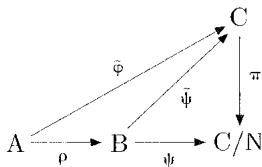
\includegraphics[keepaspectratio]{images/part001_4eedc660.jpg}}

借助 \(\tilde{\varphi}\) 把 C 与 C/N 视为 A-代数，于是 \(\psi\) 是 \(A\) -代数同态；由于 B 在 A 上形式光滑，存在连续 A-代数同态 \(\tilde{\psi}: B \to C\) 使 \(\pi \circ \tilde{\psi} = \psi\)，由此得 a)。

\begin{enumerate}
\def\labelenumi{\alph{enumi})}
\setcounter{enumi}{1}
\item
  只需证明两个形式光滑 \(k\)-代数 \(\mathrm{A}_1\) 与 \(\mathrm{A}_2\) 的乘积形式光滑。设 \(\varphi : \mathrm{A}_1 \times \mathrm{A}_2 \to \mathrm{C} / \mathrm{N}\) 为连续 \(k\)-代数同态。令 \(e_1 = \varphi(1,0)\)，\(e_2 = \varphi(0,1)\)，于是 \(e_1\) 与 \(e_2\) 是 \(\mathrm{C} / \mathrm{N}\) 中的正交幂等元。设 \(\varphi_1 : \mathrm{A}_1 \to (\mathrm{C} / \mathrm{N})e_1\) 与 \(\varphi_2 : \mathrm{A}_2 \to (\mathrm{C} / \mathrm{N})e_2\) 为由 \(\varphi_1(a_1) = \varphi(a_1,0)\) 与 \(\varphi_2(a_2) = \varphi(0,a_2)\) 定义的映射；它们是连续 \(k\)-代数同态，且有 \(\varphi(a_1,a_2) = \varphi_1(a_1) + \varphi_2(a_2)\)（对每个 \((a_1,a_2) \in \mathrm{A}_1 \times \mathrm{A}_2\)）。存在 C 的幂等元 \(\tilde{e}_1\) 使 \(\pi(\tilde{e}_1) = e_1\) (A, VIII, § 9, 第 4 节, 命题 7)；令 \(\tilde{e}_2 = 1 - \tilde{e}_1\)，于是 \(\pi(\tilde{e}_2) = e_2\)。为证这对 \(i = 1,2\) 成立：同态 \(\mathrm{C}\tilde{e}_i \to (\mathrm{C} / \mathrm{N})e_i\)（由 \(\pi\) 诱导）是满射的，核为 \(\mathrm{N}\tilde{e}_i\)；由于 \(k\)-代数 \(\mathrm{A}_i\) 形式光滑，同态 \(\varphi_i\) 有一个连续提升 \(\tilde{\varphi}_i\)（到 \(\mathrm{C}\tilde{e}_i\) 中）。映射 \((a_1,a_2) \mapsto \tilde{\varphi}_1(a_1) + \tilde{\varphi}_2(a_2)\) 是 \(\varphi\) 到 C 中的连续提升。
\item
  设 \(i: \mathrm{A} \to \widehat{\mathrm{A}}\) 为典范同态。对每个赋予离散拓扑的环 D，把连续同态 \(f: \widehat{\mathrm{A}} \to \mathrm{D}\) 对应为连续同态 \(f \circ i: \mathrm{A} \to \mathrm{D}\) 的映射是双射的。断言 c) 由此得出。
\end{enumerate}

命题的断言 c) 特别适用于 \(A\) 的拓扑是 J-进拓扑且 \(J\) 是有限生成理想的情形：此时闭包 \(\widehat{J}\)（\(J\) 在 \(\widehat{A}\) 中的）等于 \(\widehat{JA}\)，且 \(\widehat{A}\) 的拓扑是 \(\widehat{J}\)-进拓扑 (III, § 2, 第 12 节, 命题 16 的推论 2)。于是，说 \(A\) 对 J-进拓扑形式光滑，与说它的分离完备化 \(\widehat{A}\) 对 J-进拓扑形式光滑，两者等价。

命题 4.--- 设 k 为环，A 与 B 为 k-代数，J 为 A 的理想，K 为 B 的理想。

\begin{enumerate}
\def\labelenumi{\alph{enumi})}
\item
  设 S 为 A 的乘性子集，T 为 k 的其在 A 中的像含于 S 的子集。若 \(A\) 对 J-进拓扑在 \(k\) 上形式光滑，则 S \(^{-1}A\) 在 \(\mathrm{T}^{-1}k\) 上对 \(\mathrm{S}^{-1}\mathrm{J}\)-进拓扑形式光滑。
\item
  设 \(k'\) 为 \(k\)-代数。若 A 对 J-进拓扑在 \(k\) 上形式光滑，则 \(k'\)-代数 \(A_{(k')}\) 在 \(k'\) 上对 \(JA_{(k')}\)-进拓扑形式光滑。
\item
  以 I 表示 A ⊗k B 中由 J ⊗k B 与 A ⊗k K 的像生成的理想。若 A 与 B 分别对 J-进与 K-进拓扑在 k 上形式光滑，则 k-代数 A ⊗k B 对 I-进拓扑形式光滑。
\item
  在 a) 的假设下，设 C 为 \(\mathrm{T}^{-1}k\)-代数，N 为 C 中的平方零理想；赋予 C 与 C/N 以离散拓扑，并以 \(\pi : C \to C/N\) 表示典范满射。设 \(\varphi : S^{-1}A \longrightarrow C/N\) 为一个 \(\mathrm{T}^{-1}k\)-代数同态（对 \(\mathrm{S}^{-1}\mathrm{J}\)-进拓扑连续）。以 i 表示从 A 到 \(S^{-1}A\) 中的典范同态。映射 \(\varphi \circ i\) 是对 J-进拓扑连续的 k-代数同态，故有提升 \(\tilde{\varphi}_{0} : A \to C\)。\(\tilde{\varphi}_{0}(S)\) 中的元素模 N 可逆，由于 N 幂零，故它们可逆。于是存在环同态 \(\tilde{\varphi} : S^{-1}A \to C\) 使 \(\tilde{\varphi} \circ i = \tilde{\varphi}_{0}\) (II, § 2, 第 1 节, 命题 1)；由同上引文命题 2 的推论 3，\(\tilde{\varphi}\) 是 \(\mathrm{T}^{-1}k\)-线性的。我们有 \(\pi \circ \tilde{\varphi} \circ i = \varphi \circ i\)，从而 \(\pi \circ \tilde{\varphi} = \varphi\) (同上引文, 命题 1)，于是 \(\tilde{\varphi}\) 是 \(\varphi\) 的一个提升。
\item
  置身于 b) 的假设之下。设 C 为 \(k'\)-代数，N 为 C 中的平方零理想；赋予 C 与 C/N 以离散拓扑。设 \(\varphi : \mathrm{A}_{(k')} \longrightarrow \mathrm{C/N}\) 为一个 \(k'\)-代数同态（对 \(J\mathrm{A}_{(k')}\)-进拓扑连续）。以 \(i : \mathrm{A} \to \mathrm{A}_{(k')}\) 表示典范同态。映射 \(\varphi \circ i\) 是从 A 到 C/N 的、对 J-进拓扑连续的 \(k\)-代数同态；若 A 对 J-进拓扑在 \(k\) 上形式光滑，则 \(\varphi \circ i\) 有提升 \(\tilde{\psi} : \mathrm{A} \to \mathrm{C}\)。\(k'\)-代数同态 \(\tilde{\varphi} : \mathrm{A}_{(k')} \longrightarrow \mathrm{C}\)（由 \(\tilde{\psi}\) 导出）是 \(\varphi\) 的一个提升。
\item
  置身于 c) 的假设之下。由 b)，B-代数 A⊗ \(_{k}\) B 对 J(A⊗ \(_{k}\) B)-进拓扑形式光滑，从而对 I-进拓扑形式光滑；此外，当 B 赋予 K-进拓扑且 A⊗ \(_{k}\) B 赋予 I-进拓扑时，典范同态 B → A⊗ \(_{k}\) B 连续。于是断言 c) 由命题 3, a) 得出。
\end{enumerate}

\subsection{形式光滑代数的例子}

设 k 为环。

\begin{enumerate}
\def\labelenumi{\arabic{enumi})}
\tightlist
\item
  设 P 为投射 \(k\)-模。对称 \(k\)-代数 \(\mathbf{S}_k(\mathrm{P})\) 对离散拓扑形式光滑，更不必说对其分次所定义的拓扑形式光滑。事实上，对任意 \(k\)-代数 C 与 C 的每个理想 N，从 \(\mathbf{S}_k(\mathrm{P})\) 到 C（相应地 C/N）中的代数同态与从 P 到 C（相应地 C/N）中的 \(k\)-线性映射一一对应，且典范映射 \(\mathrm{Hom}_k(\mathrm{P},\mathrm{C}) \to \mathrm{Hom}_k(\mathrm{P},\mathrm{C}/\mathrm{N})\) 是满射的。
\end{enumerate}

因此 (命题 3, c))，\(k\)-代数 \(\widehat{\mathbf{S}}_k(\mathrm{P}) = \prod_{n\geqslant 0}\mathbf{S}_k^n (\mathrm{P})\) 是形式光滑的（对诸 \(\mathbf{S}_k^n (\mathrm{P}))\) 上离散拓扑的乘积拓扑）；事实上，它是 \(k\)-代数 \(\mathbf{S}_k(\mathrm{P})\) 对由分次定义的拓扑的完备化。

\begin{enumerate}
\def\labelenumi{\arabic{enumi})}
\setcounter{enumi}{1}
\item
  对任意不定元族 \(\mathbf{T} = (\mathrm{T}_i)_{i\in I}\)，多项式 \(k\)-代数 \(k[\mathbf{T}]\) 与赋予其典范拓扑的形式幂级数 \(k\)-代数 \(k[[\mathbf{T}]]\) 都是形式光滑的；这由例 1 得出。若 \(k\) 是域，则纯超越扩张 \(k(\mathbf{T})\) 形式光滑 (第 2 节, 命题 4 a))。
\item
  设 \(f \in k[\mathrm{T}]\) 为一个不定元的多项式。说 \(k\)-代数 \(k[\mathrm{T}]/(f)\) 形式光滑，就是说满足下述性质：对每个 \(k\)-代数 C 与 C 的每个平方零理想 N，\(f\) 在 C/N 中的每个根都可提升为 \(f\) 在 C 中的根。当 \(f\) 与其导数 \(f'\) 生成单位理想时即属此情形。事实上，设 \(\alpha\) 为 \(f\) 在 C/N 中的根，\(a\) 为 C 中提升 \(\alpha\) 的元素。于是 \(f(a)\) 属于 N，从而 \(f'(a)\) 在 C 中可逆；元素 \(b = a - f'(a)^{-1}f(a)\) 提升 \(\alpha\)。由于 \(f'(a)^{-1}f(a)\) 的平方为零，有
\end{enumerate}

\[
f (b) = f (a) - f ^ {\prime} (a) f ^ {\prime} (a) ^ {- 1} f (a) = 0.
\]

定理 1 (I. S. Cohen). 设 \(k\) 为域，\(K\) 为 \(k\) 的可分扩张。则 \(K\) 是形式光滑 \(k\)-代数。

设 C 为 \(k\)-代数，N 为 C 中的平方零理想，\(\pi: \mathrm{C} \to \mathrm{C/N}\) 为典范同态，\(\varphi: \mathrm{K} \to \mathrm{C/N}\) 为 \(k\)-代数同态。尚需构造 \(\varphi\) 的一个提升。我们区分两种情形。

\begin{enumerate}
\def\labelenumi{\Alph{enumi})}
\item
  先设 k 的特征为 0。考察偶 \((\mathrm{K}^{\prime}, \tilde{\varphi}^{\prime})\)，其中 \(K^{\prime}\) 是 K 的中间扩张，\(\tilde{\varphi}^{\prime}: K^{\prime} \to C\) 是 \(\varphi\) 在 \(K^{\prime}\) 上的限制的一个提升。这些偶按延拓关系排序后的集合是归纳的；由 Zorn 引理 (E, III, 第 20 页, 定理 2)，存在极大偶 \((\mathrm{K}^{\prime}, \tilde{\varphi}^{\prime})\)。我们来证明 \(K^{\prime}\) 等于 K。设 \(x \in K - K^{\prime}\)。若 x 在 \(K^{\prime}\) 上超越，则 \(K^{\prime}\)-代数 \(\mathrm{K}^{\prime}(x)\) 形式光滑 (例 2)。若 x 在 \(K^{\prime}\) 上代数，则其极小多项式 \(f \in K^{\prime}[T]\) 与其导数互素 (A, V, 第 37 页, 命题 4)，而 \(\mathrm{K}^{\prime}(x)\) 与 \(K^{\prime}\)-代数 \(\mathrm{K}^{\prime}[\mathrm{T}]/(f)\) 恒同，后者因此是形式光滑 \(K^{\prime}\)-代数 (例 3)。两种情形下，\(\mathrm{K}^{\prime}(x)\) 都在 \(K^{\prime}\) 上形式光滑，于是存在 \(\tilde{\varphi}^{\prime}\) 到 \(\mathrm{K}^{\prime}(x)\) 的一个延拓，它提升 \(\varphi\) 在 \(\mathrm{K}^{\prime}(x)\) 上的限制，这与 \((\mathrm{K}^{\prime}, \tilde{\varphi}^{\prime})\) 的极大性矛盾。
\item
  设 \(k\) 的特征为 \(p \neq 0\)。考察环同态 F: C → C，它满足 F(x) = x \(^{p}\)；对 x ∈ N 有 F(x) = 0，于是存在唯一的环同态 λ: C/N → C 使 λ ∘ π = F。有 π(λ(π(x))) = π(x \(^{p}\)) = π(x) \(^{p}\)；由于 π 满射，故对 C/N 的每个元素 z 有 π(λ(z)) = z \(^{p}\)。另一方面，设 f: K → K \(^{p}\) 为同构 y ↦ y \(^{p}\)，f \(^{-1}\): K \(^{p}\) → K 为其逆同构。设 g: K \(^{p}\) → C 为下列环同态的复合
\end{enumerate}

\[
\mathrm{K} ^ {p} \xrightarrow {f ^ {- 1}} \mathrm{K} \xrightarrow {\varphi} \mathrm{C} / \mathrm{N} \xrightarrow {\lambda} \mathrm{C}.
\]

对每个 \(x \in K\)，有 \(g(x^{p}) = \lambda(\varphi(x))\)。由于 \(\lambda(\alpha z) = \alpha^{p}\lambda(z)\)（对 \(\alpha \in k\) 与 \(z \in C/N\)），映射 \(g\) 是 \(k^{p}\)-线性的。由于 \(K\) 在 \(k\) 上的扩张可分，\(k(K^{p})\) 与 \(k \otimes_{k^{p}} K^{p}\) 恒同 (A, V, 第 119 页, 注)；于是存在唯一的 \(k\)-代数同态 \(h: k(K^{p}) \to C\)，它与 \(g\) 在 \(K^{p}\) 上重合。

设 \((a_{i})_{i\in I}\) 为 K 的一个 \(p\)-基（在 \(k(\mathrm{K}^p)\) 上）(A, V, 第 98 页, 定理 2)；对每个 \(i\in I\)，选取 C 的一个元素 \(b_{i}\)，满足 \(\pi(b_{i})=\varphi(a_{i})\)。有 \(h(a_{i}^{p})=g(a_{i}^{p})=\lambda(\varphi(a_{i}))=\lambda(\pi(b_{i}))=b_{i}^{p}\)（对每个 \(i\in I\)）。据 A, V, 第 94 页的注，存在 \(k\)-代数同态 \(\tilde{\varphi}:K\to C\)，它扩张 \(h\) 且满足 \(\tilde{\varphi}(a_{i})=b_{i}\)（对每个 \(i\)）。有 \(\pi(\tilde{\varphi}(a_{i}))=\pi(b_{i})=\varphi(a_{i})\)（对每个 \(i\)），且 \(\pi(\tilde{\varphi}(x^{p}))=\pi(h(x^{p}))=\pi(g(x^{p}))=\pi(\lambda(\varphi(x)))=\varphi(x^{p})\)（对每个 \(x\in K\)）。于是有 \(\pi\circ\tilde{\varphi}=\varphi\)，证明完毕。

推论.--- 设 k 为域，K 为 k 的可分扩张，A 为线性拓扑 K-代数。若 A 在 K 上形式光滑，则它在 k 上形式光滑。

这由定理及第 2 节的命题 3 a) 得出。

注.- 1) 设 \(k\) 为域。每个平展的 \(k\) -代数 (A, V, 第 28 页, 定义 1) 都形式光滑 (同上引文, 第 34 页, 定理 4, d) 与第 2 节, 命题 3, b))。

\begin{enumerate}
\def\labelenumi{\arabic{enumi})}
\setcounter{enumi}{1}
\tightlist
\item
  我们将在下面 (第 5 节定理 2 的推论 2) 看到：形式光滑的域扩张是绝对正则的，从而是可分的 (§ 6, 第 4 节, 例 2)。
\end{enumerate}

\subsection{完备滤过代数中同态的提升}

设 \(k\) 为环，C 为 \(k\)-代数，\((C_n)_{n \in \mathbf{Z}}\) 为 C 的递降滤过，它与 \(k\)-代数结构相容且满足 \(C_0 = C\) (III, § 2, 第 1 节)。设 C 对由此滤过定义的拓扑是分离且完备的，于是典范映射 \(C \to \varprojlim C / C_n\) 是同胚 (同上引文, 第 6 节)。设 \(m\) 为整数 \(>0\)。以 \(\pi: C \to C / C_m\) 表示典范满射。

命题 5.—设 A 为线性拓扑的形式光滑 \(k\)-代数。每个连续 \(k\)-代数同态 \(\varphi: A \to \mathrm{C/C}_{m}\) 都有到 C 中的连续提升。

对每个整数 \(n > m\)，以 \(\pi_n: \mathrm{C/C}_n \to \mathrm{C/C}_{n-1}\) 表示典范满射。由于 C 与诸 \(\mathrm{C/C}_n\) 的逆极限恒同，给出 \(\varphi\) 到 C 的连续提升，或给出一个族 \((\varphi_n)_{n > m}\)——由连续 \(k\)-代数同态 \(\varphi_n: \mathrm{A} \to \mathrm{C/C}_n\) 组成，满足 \(\pi_n \circ \varphi_n = \varphi_{n-1}\)——两者等价。于是通过对 \(m\) 用归纳法，只需在 \(\mathrm{C}_{m+1} = 0\) 时证明陈述。此时理想 \(\mathrm{C}_m\) 的平方为零（因为 \(2m \geqslant m+1\)），由于 A 形式光滑，命题得证。

例.—设 C 为 \(k\)-代数，N 为 C 的幂零理想。该命题适用于赋予 N-进滤过的代数 C。若 A 为线性拓扑的形式光滑 \(k\)-代数，我们得到：从 A 到赋予离散拓扑的 \(k\)-代数 C/N 中的每个连续同态，都可提升为从 A 到赋予离散拓扑的 \(k\)-代数 C 中的连续同态。

\subsection{代数的形式光滑商}

定理 2.--- 设 k 为环，A 为 k-代数，J 为 A 的理想且 k-代数 A/J 形式光滑。赋予 A 以 J-进拓扑。下列条件等价：

\begin{enumerate}
\def\labelenumi{(\roman{enumi})}
\item
  拓扑 k-代数 A 形式光滑；
\item
  \(A/\mathrm{J}\)-模 \(\mathrm{J}/\mathrm{J}^2\) 是投射的，且典范同态 (§ 5, 第 2 节)
\end{enumerate}

\[
\beta : \mathbf {S} _ {\mathrm{A/J}} (\mathrm{J} / \mathrm{J} ^ {2}) \rightarrow \operatorname{gr} _ {\mathrm{J}} (\mathrm{A})
\]

是双射的；

\begin{enumerate}
\def\labelenumi{(\roman{enumi})}
\setcounter{enumi}{2}
\tightlist
\item
  A/J-模 J/J \(^{2}\) 是投射的，且存在从 A 的分离完备化到分次代数 \(\mathsf{S}_{A/J}\) (J/J \(^{2}\)) 的完备化上的拓扑 k-代数同构。
\end{enumerate}

若 A 是 Noether 的，这些条件也等价于：

\begin{enumerate}
\def\labelenumi{(\roman{enumi})}
\setcounter{enumi}{3}
\tightlist
\item
  理想 J 是完全割的。
\end{enumerate}

首先注意 (iii) 蕴含 (i)：事实上，在 (iii) 的假设下，代数 \(\mathsf{S}_{\mathrm{A}/\mathrm{J}}(\mathrm{J}/\mathrm{J}^{2})\) 赋予与其分次相伴的拓扑后，在 A/J 上形式光滑 (第 3 节, 例 1)，从而在 k 上形式光滑 (第 2 节, 命题 3, a))；于是断言 (i) 由第 2 节的命题 3, c) 得出。

设 \(\widehat{\mathbf{A}}\) 为代数 A 的分离完备化，\(\widehat{\mathbf{J}}\) 为 J 的分离完备化。典范同态 \(i: \mathbf{A} \to \widehat{\mathbf{A}}\) 诱导出同构 \(\mathrm{A} / \mathrm{J} \longrightarrow \widehat{\mathrm{A}} / \widehat{\mathrm{J}}\) (III, § 2, 第 12 节, 公式 (21))。设 \(\varphi: \mathrm{A} / \mathrm{J} \to \widehat{\mathrm{A}}\) 为该同构的一个提升 (第 4 节, 命题 5)。以 \(\lambda: \widehat{\mathrm{J}} \to \mathrm{J} / \mathrm{J}^2\) 表示由典范同构 \(\mathrm{J} / \mathrm{J}^2 \longrightarrow \widehat{\mathrm{J}} / \widehat{\mathrm{J}}^2\) (III, § 2, 第 12 节, 公式 (21)) 导出的满射。设 \(a\) 为 A 的元素，\(\bar{a}\) 为它在 \(\mathrm{A} / \mathrm{J}\) 中的类，\(z\) 为 \(\widehat{\mathrm{J}}\) 的元素；有 \(\varphi(\bar{a}) \equiv i(a)\) (mod. \(\widehat{\mathrm{J}}\))，从而 \(\varphi(\bar{a})z \equiv i(a)z\) (mod. \(\widehat{\mathrm{J}}^2\))，且 \(\lambda(\varphi(\bar{a})z) = \lambda(i(a)z) = \bar{a}\lambda(z)\)。换言之，\(\lambda\) 是 A/J-线性的（当赋予 \(\widehat{\mathbf{J}}\) 由 \(\varphi\) 诱导的 A/J-模结构时）。

设同态 \(\lambda\) 有一个 A/J-线性截面 \(\sigma : J/J^{2} \longrightarrow \widehat{J}\)。设 \(S\) 为 \(k\)-分次代数 \(S_{A/J}(J/J^{2})\)，\(\widehat{S}\) 为其完备化。设

\[
\theta : \mathsf {S} \to \widehat {\mathsf {A}}
\]

为如下定义的 \(k\)-代数同态：满足 \(\theta(x) = \varphi(x)\)，其中 \(x\) 属于 \(\mathbf{S}^0 = \mathrm{A}/\mathrm{J}\)；且 \(\theta(x) = \sigma(x)\)，其中 \(x\) 属于 \(\mathbf{S}^1 = \mathrm{J}/\mathrm{J}^2\)。由于 \(\theta\) 把 \(\mathbf{S}^1\) 映入 \(\widehat{\mathbf{J}}\)，它把 \(\mathbf{S}^n\) 映入 \(\widehat{\mathbf{J}}^n\)，从而扩张为连续同态 \(\widehat{\boldsymbol{\theta}}: \widehat{\mathbf{S}} \to \widehat{\mathbf{A}}\)。映射 \(\mathrm{gr}_1(\boldsymbol{\theta}): \mathrm{J}/\mathrm{J}^2 \longrightarrow \widehat{\mathrm{J}}/\widehat{\mathrm{J}}^2\) 是 \(\sigma\) 与典范满射 \(\widehat{\mathrm{J}} \longrightarrow \widehat{\mathrm{J}}/\widehat{\mathrm{J}}^2\) 的复合；由于 \(\sigma\) 是 \(\lambda\) 的一个截面，\(\mathrm{gr}_1(\boldsymbol{\theta})\) 与从 \(\mathrm{J}/\mathrm{J}^2\) 到 \(\widehat{\mathrm{J}}/\widehat{\mathrm{J}}^2\) 上的典范同构重合。于是 \(\mathrm{gr}(\boldsymbol{\theta}): \mathbf{S} \to \mathrm{gr}_{\widehat{\mathbf{J}}}(\widehat{\mathbf{A}})\) 是典范满射 \(\beta\) 与典范同构 \(\mathrm{gr}_\mathrm{J}(\mathrm{A}) \to \mathrm{gr}_{\widehat{\mathbf{J}}}(\widehat{\mathbf{A}})\) 的复合 (III, § 2, 第 12 节, 公式 (22))。

现在证明蕴涵 (ii)⇒(iii)。在假设 (ii) 之下，A/J-模 J/J² 是投射的，故 λ 有一个 A/J-线性截面；由前面的构造与该截面相伴的同态 \(\widehat{\boldsymbol{\theta}}:\widehat{\mathbf{S}}\to\widehat{\mathbf{A}}\) 依假设在相伴分次模上诱导出同构，从而是双射 (III, § 2, 第 8 节, 定理 1 的推论 3)，这就证明了 (iii)。

我们来证明 (i)⇒(ii)。设拓扑 k-代数 A 形式光滑。首先证明 A/J-模 \(J/J^{2}\) 是投射的。设 M 为 \(A/J\)-模，\(f:M\to J/J^{2}\) 为满的 A/J-线性映射；目标是证明 f 有一个 A/J-线性截面。

设 \(\pi: A/J^{2} \to A/J\) 为典范满射。由第 2 节的注 1，存在 \(k\)-代数同构 \(\psi: A/J \oplus J/J^{2} \longrightarrow A/J^{2}\)，满足 \(\pi(\psi(y,z)) = y\) 且 \(\psi(0,z) = z\)（对 \(y \in A/J\)、\(z \in J/J^{2}\)）。考察 \(k\)-代数 (A/J) \(\oplus M\) (第 1 节, 例) 与映射 \(u: (A/J) \oplus M \to A/J^{2}\)，它满足 \(u(x,m) = \psi(x,f(m))\)。这是 \(k\)-代数的一个满同态，其核是 \(f\) 在 M 中的核，故是平方为零的幂零理想。典范满射 \(\rho: A \to A/J^{2}\) 连续；由于 A 作为拓扑 \(k\)-代数形式光滑，存在 \(k\)-代数同态 \(\tilde{\rho}: A \to (A/J) \oplus M\) 使 \(u \circ \tilde{\rho} = \rho\)。由于 \(\mathrm{pr}_{1} = \pi \circ \psi = \pi \circ u\)，有 \(\mathrm{pr}_{1} \circ \tilde{\rho} = \pi \circ u \circ \tilde{\rho} = \pi \circ \rho\)，于是 \(\mathrm{pr}_{1} \circ \tilde{\rho}\) 是 A 到 A/J 上的典范满射。因此有 \(\tilde{\rho}(J) \subset M\)，从而 \(\tilde{\rho}(J^{2}) = 0\)，于是 \(\tilde{\rho}\) 诱导出 A/J-线性映射 \(s: J/J^{2} \to M\)。有 \(u \circ \tilde{\rho} = \rho\)，且 \(\mathrm{pr}_{2} \circ \psi^{-1} \circ u(y,m) = f(m)\)（对 \(y \in A/J\) 与 \(m \in M\)）。设 \(x \in J\)，\(\bar{x}\) 为它在 \(J/J^{2}\) 中的类；有 \(f(s(\bar{x})) = f(\mathrm{pr}_{2}(\tilde{\rho}(x))) = \mathrm{pr}_{2}(\psi^{-1}(\bar{x})) = \bar{x}\)。于是 \(s\) 是 \(f\) 的一个截面。

尚需证明同态 \(\beta\) 是单射。由于 A/J-模 \(J/J^{2}\) 是投射的，\(\lambda\) 有一个 A/J-线性截面；以 \(\theta: S \to \widehat{A}\) 表示相伴的同态。同态 gr(θ) 与 \(\beta\) 恒同。设 \(m\) 为整数；以 \(\Sigma_{m}\) 表示分次 \(k\)-代数 \(S\) 模理想 \(\sum_{i > m} S^{i}\) 所得的商，以 \(\theta_{m}: \Sigma_{m} \to A/J^{m+1}\) 表示由 \(\theta\) 导出的同态。\(\theta_{m}\) 与典范满射 \(A/J^{m+1} \longrightarrow A/J\) 的复合是 \(\Sigma_{m}\) 到 \(S^{0} = A/J\) 上的典范投影；于是 \(\theta_{m}\) 的核是幂零理想。由第 4 节的例，存在一个提升 \(\psi_{m}: A \to \Sigma_{m}\)（典范满射 \(A \to A/J^{m+1}\) 的提升）。由于 \(\psi_{m}\) 与从 \(\Sigma_{m}\) 到 A/J 上的典范投影的复合是典范满射，\(\psi_{m}(J)\) 由次数 \(>0\) 的元素组成。通过过渡到相伴分次对象，我们从 \(\psi_{m}\) 得到一个 \(k\)-线性分次映射 gr(\(\psi_{m}\)): gr \(_{J}(A) \to \Sigma_{m}\)，满足 gr \(_{m}(\theta) \circ\) gr \(_{m}(\psi_{m}) = \text{Id}_{J^{m}/J^{m+1}}\)。由此推出 gr \(_{m}(\theta)\)——从而 \(\beta_{m}\) 也——是单射，这就完成了 (ii) 的证明。

最后，当 A 是 Noether 的时，条件 (ii) 与 (iv) 等价 (§ 5, 第 2 节, 定理 1)。

推论 1.--- 设 \(k\) 为域，A 为 \(k\)-局部 Noether 代数，且扩张 \(\kappa_{A}\)（在 \(k\) 上）可分。下列条件等价：

\begin{enumerate}
\def\labelenumi{(\roman{enumi})}
\item
  \(k\)-代数 A 对 \(\mathfrak{m}_{\mathrm{A}}\)-进拓扑形式光滑；
\item
  环 A 正则；
\item
  \(k\)-代数 A 绝对正则 (\(\S 6, \mathrm{n}^{\circ} 4\), 定义 1)；
\item
  k-代数 \(\hat{A}\) 同构于 \(\kappa_{A}[[T_{1},\ldots,T_{n}]]\)，其中 \(n=\dim A\)。
\end{enumerate}

条件 (ii) 与 (iii) 的等价由 § 6 第 4 节的例 3 得出，且两者等价于说理想 \(\mathfrak{m}_{\mathrm{A}}\) 是完全割的 (VIII, § 5, 第 2 节, 定理 1)。此外，\(\widehat{\mathrm{A}}\) 到 \(\kappa_{\mathrm{A}}[[\mathrm{T}_{1},\ldots,\mathrm{T}_{n}]]\) 上的每个环同构都是双连续的，因为它们都是局部环。由于 \(k\)-代数 \(\mathrm{A}/\mathfrak{m}_{\mathrm{A}}\) 形式光滑 (第 3 节, 定理 1)，取 \(\mathrm{J}=\mathfrak{m}_{\mathrm{A}}\) 应用定理 2 即得推论。

推论 2.--- 设 k 为域，A 为 Noether k-代数，J 为 A 的含于 A 的根式中的理想。设 k-代数 A 对 J-进拓扑形式光滑。则它绝对正则。

事实上，设 \(k'\) 为 \(k\) 的有限扩张，\(A'\) 为 A-代数 \(A_{(k')}\)；尚需证明：对每个极大理想 \(\mathfrak{m}'\)（\(A'\) 的），Noether 局部环 \(A_{\mathfrak{m}'}'\) 都是正则的。我们有 \(JA' \subset \mathfrak{m}'\)：事实上，\(\mathfrak{m}'\) 在 A 中的逆像是 A 的一个极大理想 (V, § 2, 第 1 节, 命题 1)，故包含 J。\(k'\)-代数 \(A'\) 对 \(JA'\)-进拓扑形式光滑 (第 2 节, 命题 4, b))，而 \(k'\)-代数 \(A_{\mathfrak{m}'}'\) 对 \(JA_{\mathfrak{m}'}'\)-进拓扑形式光滑 (第 2 节, 命题 4, a))，故对 \(\mathfrak{m}'A_{\mathfrak{m}'}'\)-进拓扑也形式光滑。设 \(k_0\) 为 \(k'\) 的素子域。则 \(A_{\mathfrak{m}'}'\) 在 \(k_0\) 上对 \(\mathfrak{m}'A_{\mathfrak{m}'}'\)-进拓扑形式光滑 (第 3 节定理 1 的推论)；由于 \(\kappa(\mathfrak{m}')\) 在 \(k_0\) 上可分，环 \(A_{\mathfrak{m}'}'\) 正则 (推论 1)。

推论 3.--- 设 k 为环，A 为形式光滑 k-代数。

\begin{enumerate}
\def\labelenumi{\alph{enumi})}
\item
  A-模 \(\Omega_k(A)\) 是投射的。
\item
  设环 A ⊗k A 是 Noether 的。设 μ : A ⊗k A → A 为满足 μ(x ⊗ y) = xy 的同态；则理想 Ker(μ) 是完全割的。
\end{enumerate}

\(k\)-代数 A 与 \(\mathbf{A} \otimes_{k} \mathbf{A}\) 形式光滑 (第 2 节, 命题 4, c))，且 A 同构于 \(\mathbf{A} \otimes_{k} \mathbf{A}\) 模 \(\mu\) 的核 I 所得的商。依定义，\(\Omega_{k}(\mathbf{A}) = \mathbf{I}/\mathbf{I}^{2}\)。于是 a) 与 b) 由定理 2 得出。

\subsection{正则代数中基域的扩张（特征非零）}

设 \(k\) 为环，\(\rho: A \to B\) 为 \(k\)-代数同态。同态 \(\rho\) 诱导出 A-线性映射 \(\Omega(\rho): \Omega_k(A) \to \Omega_k(B)\)，从而诱导出 B-线性映射 \(\Omega_0(\rho): B \otimes_A \Omega_k(A) \to \Omega_k(B)\) (A, III, 第 135 页)。设 \(\mathbf{T} = (\mathrm{T}_i)_{i \in I}\) 为不定元族，\(\mathbf{t} = (t_i)_{i \in I}\) 为 B 的元素族；对每个多项式 \(f = \sum_{\alpha \in \mathbf{N}^{(I)}} c_\alpha \mathbf{T}^\alpha\)（A{[} \(\mathbf{T}\) {]} 中的），以 \(d^{A} f(\mathbf{t})\) 表示元素 \(\sum_{\alpha} \mathbf{t}^\alpha \otimes dc_\alpha\)（\(B \otimes_A \Omega_k(A)\) 中的）。

引理 1.—设 A-代数 B 有一个生成元族 \(\mathbf{t} = (t_i)_{i\in I}\)，它们满足关系 \(f_\lambda \in \mathrm{A}[\mathbf{T}]\)（\(\lambda \in \Lambda\)）。则 B-线性同态

\[
\psi : (\mathrm{B} \otimes_ {\mathrm{A}} \Omega_ {k} (\mathrm{A})) \oplus \mathrm{B} ^ {(\mathrm{I})} \longrightarrow \Omega_ {k} (\mathrm{B})
\]

由 \(\psi(\alpha,(b_i)) = \Omega_0(\rho)(\alpha) + \sum_{i\in I}b_i\,dt_i\) 定义的映射是满射；其核由诸元素 \(n_{\lambda} = \left(d^{A}f_{\lambda}(\mathbf{t}),\left(\frac{\partial f_{\lambda}}{\partial\mathrm{T}_{i}}(\mathbf{t})\right)_{i\in I}\right)\)（\(\lambda \in \Lambda\)）生成。

考察 B-模与 B-线性映射的序列

\[
\mathrm{B} ^ {(\Lambda)} \xrightarrow {\varphi} (\mathrm{B} \otimes_ {\mathrm{A}} \Omega_ {k} (\mathrm{A})) \oplus \mathrm{B} ^ {(\mathrm{I})} \xrightarrow {\psi} \Omega_ {k} (\mathrm{B}) \longrightarrow 0,
\]

其中 \(\varphi\) 是满足 \(\varphi(e_{\lambda}) = n_{\lambda}\) 的同态；尚需证明该序列是正合的。由 A, II, 第 36 页, 定理 1，只需证明：对每个 B-模 M，序列

\[
0 \to \operatorname{Hom} _ {\mathrm{B}} (\Omega _{k}(\mathrm{B}), \mathrm{M}) \xrightarrow {\operatorname{Hom}(\psi,1)} \operatorname{Hom} _{\mathrm{B}} ((\mathrm{B} \otimes_{\mathrm{A}} \Omega _{k}(\mathrm{A})) \oplus \mathrm{B}^{(\mathrm{I})}, \mathrm{M}) \xrightarrow {\operatorname{Hom}(\varphi,1)} \operatorname{Hom}_{\mathrm{B}}(\mathrm{B}^{(\Lambda)}, \mathrm{M})
\]

是正合的。鉴于微分模的泛性质 (A, III, 第 134 页)，该序列与

\[
0 \to \mathrm{D} _ {k} (\mathrm{B}, \mathrm{M}) \xrightarrow {\psi^ {\prime}} \mathrm{D} _ {k} (\mathrm{A}, \mathrm{M}) \oplus \mathrm{M} ^ {\mathrm{I}} \xrightarrow {\varphi^ {\prime}} \mathrm{M} ^ {\Lambda}
\]

恒同，其中 \(\psi^{\prime}(\mathrm{D}) = (\mathrm{D}\circ \rho,(\mathrm{D}(t_{i}))_{i\in I})\)，\(\varphi^{\prime}(\Delta,(m_{i})) = \big(f_{\lambda}^{\Delta}(\mathbf{t}) + \sum_{i}\frac{\partial f_{\lambda}}{\partial\mathrm{T}_{i}}(\mathbf{t})m_{i}\big)_{\lambda \in \Lambda}\)（依照 A, V, 第 121 页，对每个多项式 \(f = \sum_{\alpha \in \mathbf{N}^{(I)}}c_{\alpha}\mathbf{T}^{\alpha}\)（A{[}T{]} 中的），以 \(f^{\Delta}(\mathbf{t})\) 表示元素 \(\sum_{\alpha}\mathbf{t}^{\alpha}\Delta(c_{\alpha})\)）。该序列的正合性由同上引文命题 1 得出，并注意到：导子 D : B → M 是 \(k\)-线性的，必须且只需 \(D\circ\rho\) 如此。

设 A 为环。A 上存在唯一的 \(\mathbf{Z}\)-代数结构；我们以 \(\Omega(A)\) 简记 A-模 \(\Omega_{\mathbf{Z}}(\mathrm{A})\)。若 \(\rho : k \to \mathrm{A}\) 是环同态，则有 A-模的典范正合序列 (A, III, 第 136 页, 命题 21) \(\mathrm{A} \otimes_k \Omega(k) \to \Omega(\mathrm{A}) \to \Omega_k(\mathrm{A}) \to 0\)。

设 A 包含一个子域，并设 P 为 A 的素子域；则 \(\Omega(\mathrm{P})\) 为零，且 A-模的典范同态 \(\Omega(\mathrm{A}) \to \Omega_{\mathrm{P}}(\mathrm{A})\) 是双射。若此外 A 的特征为 \(p \neq 0\)（依定义，这表示 \(p\) 是素数，\(p1_{\mathrm{A}} = 0\)，且 \(1_{\mathrm{A}} \neq 0\)），则 P 与 \(\mathbf{F}_p\) 恒同。此外，A 的每个导子都在子环 \(\mathbf{A}^p\) 上为零；对 A 的每个子环 \(k\)（含于 \(\mathbf{A}^p\) 中的；特别地，对 A 的每个完全域 \(k\)），典范映射 \(\Omega(\mathrm{A}) \to \Omega_k(\mathrm{A})\) 是双射。

设 A 为特征 \(p \neq 0\) 的环，\((f_i)_{1 \leqslant i \leqslant n}\) 为 A 的元素的一个有限序列。以 \(A_n\) 表示多项式环 \(A[T_1, \ldots, T_n]\) 模由多项式 \(T_i^p - f_i\)（\(1 \leqslant i \leqslant n\)）生成的理想所得的商环。

引理 2.—设环 A 是局部的且 Noether 的。则 \(A_{n}\) 是局部的且 Noether 的。下列条件等价：

\begin{enumerate}
\def\labelenumi{(\roman{enumi})}
\item
  \(A_{n}\) 正则；
\item
  A 正则，且元素 \(1 \otimes df_{i}\)（\(\kappa_{A}\)-向量空间 \(\kappa_{A} \otimes_{A} \Omega(A)\) 中的）线性无关。
\end{enumerate}

环 \(A_{n}\) 是 Noether 的 (III, § 2, 定理 2 的推论 3)。A-模 \(A_{n}\) 是自由的，故是忠实平坦的；若 \(A_{n}\) 正则，则 A 正则 (§ 4, 第 5 节, 命题 8 b))。我们对 n 用归纳法推理，引理在 n = 0 时是显然的。

\begin{enumerate}
\def\labelenumi{\Alph{enumi})}
\tightlist
\item
  先处理 n = 1 的情形，令 \(T_{1} = T\)，\(f_{1} = f\)。以 a 表示 f 在 \(\kappa_{A}\) 中的类，并区分两种情形：a 属于或不属于 \(\kappa_{A}^{p}\)。若 \(a \notin \kappa_{A}^{p}\)，则多项式 \(T^{p} - a\) 在 \(\kappa_{A}\) 中不可约 (A, V, 第 24 页, 引理 1)，而 \(\kappa_{A} \otimes_{A} A_{1}\) 同构于域 \(\kappa_{A}[T]/(T^{p} - a)\)。于是理想 \(m_{A}A_{1}\)（\(A_{1}\) 的）是极大的，从而环 \(A_{1}\) 是局部的 (V, § 2, 第 1 节, 命题 1)。若 A 正则，则 \(A_{1}\) 正则 (VIII, § 5, 第 1 节, 命题 1)。据 A, V, 第 99 页, 命题 6，\(\Omega(\kappa_{A})\) 中的元素 da 不为零；由于它是典范映射 \(\kappa_{A} \otimes_{A} \Omega(A) \to \Omega(\kappa_{A})\) 下 \(1 \otimes df\) 的像，后者不为零。这就在此情形证明了引理。
\end{enumerate}

现在设 \(a\) 属于 \(\kappa_{\mathrm{A}}^{p}\)。于是存在 A 的元素 \(g\) 使 \(f - g^{p} \in \mathfrak{m}_{\mathrm{A}}\)。令 \(h = f - g^{p}\)。由于 \(\mathrm{T}^{p} - f = (\mathrm{T} - g)^{p} - h\)，A-代数 \(A_{1}\) 同构于 \(\mathrm{A}[\mathrm{T}] / (\mathrm{T}^{p} - h)\)。据 VIII, § 5, 第 4 节, 命题 4，环 \(A_{1}\) 是局部的，且为使它正则，必须且只需 A 正则且 \(h\) 不属于 \(\mathfrak{m}_{\mathrm{A}}^{2}\)。而由于 \(\kappa_{A}\) 在素域上形式光滑 (第 3 节, 定理 1)，典范映射

\[
\bar {d}: \mathfrak {m} _ {\mathrm{A}} / \mathfrak {m} _ {\mathrm{A}} ^ {2} \to \kappa_ {\mathrm{A}} \otimes_ {\mathrm{A}} \Omega (\mathrm{A})
\]

是单射 (第 2 节, 注 1)；而 \(\bar{d}\) 把 \(h\) 模 \(\mathfrak{m}_{\mathrm{A}}^{2}\) 的类映为 \(1 \otimes dh = 1 \otimes d(f - g^{p}) = 1 \otimes df\)。这就在第二种情形证明了引理，并完成了 \(n = 1\) 情形的证明。

\begin{enumerate}
\def\labelenumi{\Alph{enumi})}
\setcounter{enumi}{1}
\tightlist
\item
  设 \(n > 1\)。环 \(\mathrm{A}_{1}\) 由已处理的情形是局部的且 Noether 的。\(\mathrm{A}_{1}\)-代数 \(\mathrm{A}_{n}\) 与 \(\mathrm{A}_{1}[\mathrm{T}_{2},\ldots ,\mathrm{T}_{n}]\) 模由诸 \(\mathrm{T}_i^p -f_i\)（\(i\geqslant 2\)）生成的理想所得的商恒同；由归纳假设，它是一个局部环，且条件 (i) 等价于下列两个条件的合取：
\end{enumerate}

(i') A \(_{1}\) 正则；

(i'\,') 元素 \(1 \otimes df_2, \ldots, 1 \otimes df_n\)（\(\kappa_{\mathrm{A}_1}\)-向量空间 \(\kappa_{\mathrm{A}_1} \otimes_{\mathrm{A}_1} \Omega(\mathrm{A}_1)\) 中的）线性无关。

而 (i') 由刚才所见等价于

(ii') A 正则，且元素 \(1 \otimes df_{1}\)（\(\kappa_{A}\)-向量空间 \(\kappa_{A} \otimes_{A} \Omega(A)\) 中的）不为零。

由引理 1，典范同态 \(\mathrm{A}_{1} \otimes_{\mathrm{A}} \Omega(\mathrm{A}) \to \Omega(\mathrm{A}_{1})\) 诱导出 \(((\mathrm{A}_{1} \otimes_{\mathrm{A}} \Omega(\mathrm{A})) / \mathrm{A}_{1}(1 \otimes df_{1})) \oplus \mathrm{A}_{1}\) 到 \(\Omega(\mathrm{A}_{1})\) 上的一个同构，从而诱导出 \((\kappa_{\mathrm{A}_{1}} \otimes_{\mathrm{A}} \Omega(\mathrm{A})) / \kappa_{\mathrm{A}_{1}}(1 \otimes df_{1})\) 到 \(\kappa_{\mathrm{A}_{1}} \otimes_{\mathrm{A}_{1}} \Omega(\mathrm{A}_{1})\) 中的一个单同态。由于 \(\kappa_{\mathrm{A}_{1}} \otimes_{\mathrm{A}} \Omega(\mathrm{A})\) 与 \(\kappa_{\mathrm{A}_{1}} \otimes_{\kappa_{\mathrm{A}}} (\kappa_{\mathrm{A}} \otimes_{\mathrm{A}} \Omega(\mathrm{A}))\) 恒同，断言 (i'') 于是等价于：

(ii'') 元素 \(1 \otimes df_2, \ldots, 1 \otimes df_n\) 在 \((\kappa_{\mathrm{A}} \otimes_{\mathrm{A}} \Omega(\mathrm{A})) / \kappa_{\mathrm{A}}(1 \otimes df_1)\) 中线性无关。

而 (ii') 与 (ii'') 的合取等价于 (ii)，这就证明了引理。

命题 6. 设 \(k\) 为特征 \(p \neq 0\) 的域，\(k'\) 为 \(k\) 的一个有限次且高度 \(\leqslant 1\) 的纯不可分扩张，A 为局部正则 \(k\)-代数。则 \(\mathrm{A}_{(k')}\) 是局部环，且下列条件等价：

\begin{enumerate}
\def\labelenumi{(\roman{enumi})}
\item
  环 \(A_{(k')}\) 正则；
\item
  \(\kappa_{A}\)-线性映射
\end{enumerate}

\[
\kappa_ {\mathrm{A}} \otimes_ {k ^ {\prime p}} \Omega_ {k ^ {p}} (k ^ {\prime p}) \longrightarrow \kappa_ {\mathrm{A}} \otimes_ {\mathrm{A}} \Omega (\mathrm{A})
\]

由典范单射 \(k^{\prime p}\to \mathrm{A}\) 导出的映射是单射。

实际上，设 \((x_{i})_{i\in \mathrm{I}}\) 为一个有限 \(p\)-基（\(k'\) 在 \(k\) 上的） (A, V, 第 98 页)；对每个 \(i\in \mathrm{I}\)，令 \(f_{i} = x_{i}^{p}\in k\)。\(k\)-代数 \(k'\) 与 \(k[(\mathrm{T}_i)_{i\in \mathrm{I}}]\) 模由多项式 \(\mathrm{T}_i^p - f_i\) 生成的理想所得的商恒同，因而 A-代数 \(\mathrm{A}_{(k')}\) 是 \(\mathrm{A}[(\mathrm{T}_i)_{i\in \mathrm{I}}]\) 模由多项式 \(\mathrm{T}_i^p - f_i1_{\mathrm{A}}\) 生成的理想所得的商。

此外，\((f_{i})_{i\in\mathrm{I}}\) 是 \(k^{\prime p}\) 在 \(k^{p}\) 上的一个 p-基，且 \(k^{\prime p}\)-向量空间 \(\Omega_{k^{p}}(k^{\prime p})\) 以诸 \(df_{i}\) 组成的族为一个基 (A, V, 第 97 页, 定理 1)。命题 6 于是由引理 2 得出。

\subsection{形式光滑局部代数的一个判别法}

命题 7. 设 \(k_{0}\) 为环，\(k\) 为 \(k_{0}\)-代数，A 为 \(k\)-代数，\(\mathfrak{m}\) 为 A 的一个极大理想。假设 \(k\) 与 A/\(\mathfrak{m}\) 都在 \(k_{0}\) 上形式光滑。为使 A 在 \(k\) 上对 \(\mathfrak{m}\)-进拓扑形式光滑，必须且只需下列两个条件成立：

\begin{enumerate}
\def\labelenumi{(\roman{enumi})}
\item
  典范同态 \(\mathsf{S}_{\mathrm{A} / \mathfrak{m}}(\mathfrak{m} / \mathfrak{m}^{2})\to \mathrm{gr}_{\mathfrak{m}}(\mathrm{A})\) 是双射；
\item
  A/m-线性映射
\end{enumerate}

\[
\omega : \mathrm{A} / \mathfrak {m} \otimes_ {k} \Omega_ {k _ {0}} (k) \longrightarrow \mathrm{A} / \mathfrak {m} \otimes_ {\mathrm{A}} \Omega_ {k _ {0}} (\mathrm{A})
\]

由典范映射 \(k \to A\) 导出，是单射。

设 \(d_{k}:k\to \Omega_{k_{0}}(k)\) 与 \(d_{\mathrm{A}}:\mathrm{A}\to \Omega_{k_0}(\mathrm{A})\) 为泛 \(k_{0}\)-导子。

先设 A 在 \(k\) 上对 \(\mathfrak{m}\)-进拓扑形式光滑。则 A 在 \(k_{0}\) 上对 \(\mathfrak{m}\)-进拓扑形式光滑（\(n^{\circ} 2\), 命题 3, a)），这等价于 (i)（\(n^{\circ} 5\), 定理 2）。此外，\(k_{0}\)-导子 \(\lambda \mapsto 1 \otimes d_{k}(\lambda)\)（\(k\) 的、取值于 \(A/\mathfrak{m} \otimes_{k} \Omega_{k_{0}}(k)\) 中的）可以扩张为一个 \(k_{0}\)-导子（A 的、取值于 \(A/\mathfrak{m} \otimes_{k} \Omega_{k_{0}}(k)\) 中的）（\(n^{\circ} 2\), 注 2）。于是存在 A-线性映射 \(u: \Omega_{k_{0}}(A) \to A/\mathfrak{m} \otimes_{k} \Omega_{k_{0}}(k)\)，满足 \(u(d_{A}(\lambda 1_{A})) = 1 \otimes d_{k}(\lambda)\)（对每个 \(\lambda \in k\)）。\(A/\mathfrak{m}\)-线性映射 \(A/\mathfrak{m} \otimes_{A} \Omega_{k_{0}}(A) \longrightarrow A/\mathfrak{m} \otimes_{k} \Omega_{k_{0}}(k)\)（由 \(u\) 导出）是 \(\omega\) 的一个收缩，这就证明了 (ii)。

反之，设条件 (i) 与 (ii) 成立。则 A 在 \(k_{0}\) 上对 \(\mathfrak{m}\)-进拓扑形式光滑（\(n^{\circ}5\), 定理 2），且 A-模 \(\Omega_{k_{0}}(A)\) 是投射的（\(n^{\circ}5\), 定理 2 的推论 3）。取定一个整数 \(r \geqslant 0\)，并考虑 \(A/\mathfrak{m}^{r}\)-线性映射

\[
\omega_ {r}: \mathrm{A} / \mathfrak {m} ^ {r} \otimes_ {k} \Omega_ {k _ {0}} (k) \longrightarrow \mathrm{A} / \mathfrak {m} ^ {r} \otimes_ {\mathrm{A}} \Omega_ {k _ {0}} (\mathrm{A})
\]

由典范映射 \(k\to\mathrm{A}\) 导出。设 \((\lambda_{i})_{i\in\mathrm{I}}\) 为 \(k\) 的一个元素族，使诸 \(d_{k}(\lambda_{i})\) 构成 \(k\)-向量空间 \(\Omega_{k_{0}}(k)\) 的一个基。由 (ii)，元素 \(1 \otimes d_{A}(\lambda_{i}1_{A})\) 在 A/m \(\otimes_{\mathrm{A}} \Omega_{k_0}(\mathrm{A})\) 中线性无关。据 II, § 3, 第 2 节, 命题 5 的推论 1 与 2，诸 \(1 \otimes d_{A}(\lambda_{i}1_{A})\) 构成 A/m \(^{r}\)-模 A/m \(^{r} \otimes_{\mathrm{A}} \Omega_{k_0}(\mathrm{A})\) 的一个直和项的基。于是存在一个 A/m \(^{r}\)-线性映射

\[
u _ {r}: \mathrm{A} / \mathfrak {m} ^ {r} \otimes_ {\mathrm{A}} \Omega_ {k _ {0}} (\mathrm{A}) \longrightarrow \mathrm{A} / \mathfrak {m} ^ {r} \otimes_ {k} \Omega_ {k _ {0}} (k)
\]

满足 \(u_r(1 \otimes d_A(\lambda_i 1_A)) = 1 \otimes d_k(\lambda_i)\)（对每个 \(i\)），因而 \(u_r \circ \omega_r = \mathrm{Id}\)。

现在来验证 A 在 \(k\) 上对 m-进拓扑形式光滑。设 C 为 \(k\)-代数，N 为 C 中的平方零理想，\(\pi: C \to C/N\) 为典范满射；赋予 C 与 C/N 以离散拓扑。设 \(\varphi: A \to C/N\) 为连续 \(k\)-代数同态。由于 A 在 \(k_0\) 上对 m-进拓扑形式光滑，存在连续 \(k_0\)-代数同态 \(\tilde{\varphi}_0: A \to C\)，满足 \(\pi \circ \tilde{\varphi}_0 = \varphi\)。据第 1 节的命题 1，\(k_0\)-代数同态 \(\tilde{\varphi}: A \to C\)（满足 \(\pi \circ \tilde{\varphi} = \varphi\) 者）恰是形如 \(x \mapsto v(d_A(x)) + \tilde{\varphi}_0(x)\) 的映射，其中 \(v\) 取遍 \(\mathrm{Hom}_{A}(\Omega_{k_0}(A), N)\)。尚需选取 \(v\)，使 \(\tilde{\varphi}\) 是 \(k\)-代数同态。映射 \(\lambda \mapsto \lambda 1_C - \tilde{\varphi}_0(\lambda 1_A)\) 是一个 \(k_0\)-导子（自 \(k\) 到 N 中）(同上引文)，从而可写成 \(h \circ d_k\)，其中 \(h \in \mathrm{Hom}_k(\Omega_{k_0}(k), N)\)。

取一个整数 \(r\) 使 \(\varphi\) 的核包含 \(\mathfrak{m}^r\)。A-模 N 被 \(\mathfrak{m}^r\) 零化，只需取 \(v\) 为下列同态序列的复合

\[
\Omega_ {k _ {0}} (\mathrm{A}) \longrightarrow \mathrm{A} / \mathfrak {m} ^ {r} \otimes_ {\mathrm{A}} \Omega_ {k _ {0}} (\mathrm{A}) \xrightarrow {u _ {r}} \mathrm{A} / \mathfrak {m} ^ {r} \otimes_ {k} \Omega_ {k _ {0}} (k) \xrightarrow {h ^ {\prime}} \mathrm{N},
\]

其中 \(h'\) 由 \(h\) 导出。实际上，我们有（对 \(\lambda \in k\)）：

\[
v \left(d _ {\mathrm{A}} \left(\lambda 1 _ {\mathrm{A}}\right)\right) = h ^ {\prime} u _ {r} \left(1 \otimes d _ {\mathrm{A}} \left(\lambda 1 _ {\mathrm{A}}\right)\right) = h ^ {\prime} \left(1 \otimes d _ {k} (\lambda)\right) = h \left(d _ {k} (\lambda)\right) = \lambda 1 _ {\mathrm{C}} - \tilde {\varphi} _ {0} \left(\lambda 1 _ {\mathrm{A}}\right).
\]

注 1.—当 A 为 Noether 环时，条件 (i) 表示局部环 \(A_{\mathfrak{m}}\) 是正则的 (VIII, § 5, 第 2 节, 定理 1)。

命题 8. 设 \(k\) 为域，A 为 Noether 局部 \(k\)-代数。下列条件等价：

\begin{enumerate}
\def\labelenumi{(\roman{enumi})}
\item
  A 在 \(k\) 上对 \(\mathfrak{m}_{A}\)-进拓扑形式光滑；
\item
  A 正则，且 \(\kappa_{\mathrm{A}}\)-线性映射
\end{enumerate}

\[
\omega : \kappa_ {\mathrm{A}} \otimes_ {k} \Omega (k) \longrightarrow \kappa_ {\mathrm{A}} \otimes_ {\mathrm{A}} \Omega (\mathrm{A})
\]

由典范单射 k → A 导出，是单射；

\begin{enumerate}
\def\labelenumi{(\roman{enumi})}
\setcounter{enumi}{2}
\item
  A 绝对正则；
\item
  对每个纯不可分扩张 \(k'\)（\(k\) 的、有限次且高度 \(\leqslant 1\) 的），局部环 \(A_{(k')}\) 是正则的。
\item
  (ii) \(\Leftrightarrow\) (i)：只需应用命题 7 与上面的注 1，取 \(k_{0}\) 为 \(k\) 的素子域；实际上，\(k\) 与 \(\kappa_{\mathrm{A}}\) 都在 \(k_{0}\) 上形式光滑（\(n^{\circ}3\), 参见定理 1）。
\end{enumerate}

(i)⇒(iii)：这由定理 2 的推论 2（第 5 节）得出。

(iii)⇒(iv)：这由 § 6 第 4 节的定义 1 得出。

若 \(k\) 的特征为 0，则由定理 2 的推论 1（第 5 节）可知 (iv) 蕴含 (i)，从而命题在此情形得证。设 \(k\) 的特征为 \(p \neq 0\)，证明 (iv)⇒(ii)。设 \(k'\) 为 \(k\) 的一个有限次且高度 \(\leqslant 1\) 的纯不可分扩张。若 A 与 \(\mathrm{A}_{(k')}\) 都正则，则典范映射 \(\kappa_{\mathrm{A}} \otimes_{k'^{p}} \Omega_{k^{p}}(k'^{p}) \longrightarrow \kappa_{\mathrm{A}} \otimes_{\mathrm{A}} \Omega(\mathrm{A})\) 是单射（第 6 节, 命题 6）。据 A, V, 第 97 页, 定理 1 b)（应用于扩张 \(k\)（\(k^{p}\) 上的）），\(k\)-向量空间 \(\Omega(k)\)（它与 \(\Omega_{k^{p}}(k)\) 重合）是诸子空间 \(k \otimes_{k'^{p}} \Omega_{k^{p}}(k'^{p})\) 的递增滤过并，其中 \(k'\) 取遍 \(k\) 的、高度 \(\leqslant 1\) 的有限纯不可分扩张（含于 \(k\) 的一个固定代数闭包中的）。断言 (ii) 由此得出。

注 2.—设 \(k\) 为域，A 为一个 \(k\)-代数，使得环 \(\mathrm{A}_{(k')}\) 对每个纯不可分扩张 \(k'\)（\(k\) 的、有限次且高度 \(\leqslant 1\) 的）都是正则的；则 A 绝对正则。实际上，设 \(k'\) 是这样一个扩张；对 A 的每个极大理想 \(\mathfrak{m}\)，环 \(k'\otimes_k\mathrm{A}_{\mathfrak{m}}\) 与 \(\mathrm{A}_{(k')}\) 的一个分式环恒同，因而是正则的。由上面的命题 8 与 § 6 第 4 节的命题 6，代数 A 绝对正则。

\subsection{线性映射的收缩的存在性}

命题 9. 设 A 为环，M 为有限生成 A-模，N 为投射 A-模，u : M → N 为 A-线性映射。

\begin{enumerate}
\def\labelenumi{\alph{enumi})}
\tightlist
\item
  设 p 为 A 的素理想。下列条件等价：
\end{enumerate}

\begin{enumerate}
\def\labelenumi{(\roman{enumi})}
\item
  存在 \(f \in \mathrm{A} - \mathfrak{p}\) 与 \(v \in \operatorname{Hom}_{\mathrm{A}_f}(\mathrm{N}_f, \mathrm{M}_f)\)，满足 \(v \circ u_f = \operatorname{Id}_{\mathrm{M}_f}\)；
\item
  存在 \(v \in \operatorname{Hom}_{\mathrm{A}_{\mathfrak{p}}}(\mathrm{N}_{\mathfrak{p}}, \mathrm{M}_{\mathfrak{p}})\)，满足 \(v \circ u_{\mathfrak{p}} = \operatorname{Id}_{\mathrm{M}_{\mathfrak{p}}}\)；
\item
  \(\kappa(\mathfrak{p})\text{-线性映射 }1 \otimes u : \kappa(\mathfrak{p}) \otimes_{\mathrm{A}} \mathrm{M} \to \kappa(\mathfrak{p}) \otimes_{\mathrm{A}} \mathrm{N}\) 是单射；
\item
  存在一个整数 \(m \geqslant 0\)、M 的元素 \(x_{1}, \ldots, x_{m}\) 以及 N 上的线性形式 \(y_{1}, \ldots, y_{m}\)，使得诸 \(x_{i}\) 在 \(\mathrm{M}_{\mathfrak{p}}\) 中的像生成 \(\mathrm{A}_{\mathfrak{p}}\)-模 \(\mathrm{M}_{\mathfrak{p}}\)，且 \(\det(<y_{j}, u(x_{i})>) \notin \mathfrak{p}\)；
\end{enumerate}

若条件 (iv) 成立，则有 \(m = [\kappa(\mathfrak{p}) \otimes_{\mathrm{A}} \mathrm{M} : \kappa(\mathfrak{p})]\)，且元素 \(1 \otimes x_i\) 构成 \(\kappa(\mathfrak{p})\)-向量空间 \(\kappa(\mathfrak{p}) \otimes_{\mathrm{A}} \mathrm{M}\) 的一个基。

\begin{enumerate}
\def\labelenumi{\alph{enumi})}
\setcounter{enumi}{1}
\tightlist
\item
  满足 a) 中条件的 A 的素理想 p 组成的集合 U 是 Spec(A) 的一个开子集，且下列条件等价：
\end{enumerate}

\begin{enumerate}
\def\labelenumi{(\roman{enumi})}
\item
  我们有 U = Spec(A)；
\item
  U 包含 A 的所有极大理想；
\item
  存在 \(v \in \operatorname{Hom}_{\mathrm{A}}(\mathrm{N}, \mathrm{M})\)，满足 \(v \circ u = \operatorname{Id}_{\mathrm{M}}\)；
\item
  u 是单射，且 Coker(u) 是投射 A-模。
\end{enumerate}

我们来证明 a)。

(i)⇒(ii)⇒(iii)：这些蕴含关系是显然的。

(iii)⇒(iv)：令 \(m = [\kappa(\mathfrak{p}) \otimes_{\mathrm{A}} \mathrm{M} : \kappa(\mathfrak{p})]\)，设 \((x_{1}, \ldots, x_{m})\) 为 M 的元素序列，使元素 \(1 \otimes x_{i}\) 构成 \(\kappa(\mathfrak{p})\)-向量空间 \(\kappa(\mathfrak{p}) \otimes_{\mathrm{A}} \mathrm{M}\) 的一个基。由 Nakayama 引理，诸 \(x_{i}\) 在 \(M_{p}\) 中的像生成 \(A_{p}\)-模 \(M_{p}\)。若条件 (iii) 成立，则元素 \(1 \otimes u(x_{i})\)（\(\kappa(\mathfrak{p})\)-向量空间 \(\kappa(\mathfrak{p}) \otimes_{\mathrm{A}} N\) 中的）线性无关。

此外，存在一个 A-模 \(N'\)、一个指标集 I，以及 A-模的同构 \(\theta : N \oplus N' \to \mathrm{A}^{(\mathrm{I})}\)，由此导出 \(\kappa(\mathfrak{p})\)-向量空间的一个同构

\[
\overline {{{\theta}}}: (\kappa (\mathfrak {p}) \otimes_ {\mathrm{A}} N) \oplus (\kappa (\mathfrak {p}) \otimes_ {A} N ^ {\prime}) \rightarrow \kappa (\mathfrak {p}) ^ {(I)}.
\]

元素 \(t_i = \bar{\theta}(1 \otimes u(x_i), 0)\)（\(\kappa(\mathfrak{p})^{(I)}\) 中的）构成一个有限自由族。于是存在 I 的元素 \(\alpha_1, \ldots, \alpha_{m}\)，使得 \(\det(\mathrm{pr}_{\alpha_j}(t_i)) \neq 0\)；N 上的线性形式 \(y_j : z \mapsto \mathrm{pr}_{\alpha_j}(\theta(z, 0))\) 即合要求。

设条件 (iv) 成立。以 \((a_{ij}) \in \mathbf{M}_m(\mathrm{A})\) 表示由系数 \(a_{ij} = \langle y_j, u(x_i)\rangle\) 组成的矩阵。设 \(g\) 为 \(\mathrm{A} - \mathfrak{p}\) 的元素，使诸 \(x_i\) 的像生成 \(\mathrm{A}_g\)-模 \(\mathrm{M}_g\) (II, § 5, 第 1 节, 命题 2)，并令 \(f = g \det(a_{ij})\)。由于 \(\det(a_{ij})\) 在 \(\mathrm{A}_f\) 中可逆，元素 \(u(x_i)\) 在 \(\mathrm{N}_f\) 中的像线性无关；因而诸 \(x_i\) 在 \(\mathrm{M}_f\) 中的像构成这个 \(\mathrm{A}_f\)-模的一个基。这就证明了 a) 的最后一个断言。现在证明 (i)。以 \(w \in \operatorname{Hom}_{\mathrm{A}}(\mathrm{N}, \mathrm{M})\) 表示映射 \(z \mapsto \sum_{j} \langle y_j, z\rangle x_j\)。我们有

\[
w \circ u (x _ {i}) = \sum_ {j} a _ {i j} x _ {j};
\]

由于诸 \(x_{i}\) 的像构成 \(M_{f}\) 的一个基，且矩阵 \((a_{ij})\) 在 \(\mathbf{M}_{m}(\mathrm{A}_{f})\) 中可逆，\((w \circ u)_{f}\)（\(M_{f}\) 的自同态）是双射的，而映射 \(v = (w \circ u)_{f}^{-1} \circ w_{f} \in \operatorname{Hom}_{\mathrm{A}_{f}}(\mathrm{N}_{f}, \mathrm{M}_{f})\) 满足条件 (i)。

我们来证明 b)。U 是开集这一事实由 a) 的条件 (i) 得出。

(iii)⇒(i)⇒(ii)：这是显然的。

(iv)⇒(iii)：在 (iv) 的假设下，序列 0 → M \(\xrightarrow{u}\) N \(\longrightarrow\) Coker(u) → 0 是正合且分裂的，故得 (iii)。

\begin{enumerate}
\def\labelenumi{(\roman{enumi})}
\setcounter{enumi}{1}
\tightlist
\item
  (ii) \(\Rightarrow\) (iv)：如上引入一个 A-模同构 \(\theta: \mathrm{N} \oplus \mathrm{N}' \to \mathrm{A}^{(\mathrm{I})}\)。设 \(u'\) 为从 M 到 \(\mathrm{A}^{(\mathrm{I})}\) 中的映射（由 \(u'(x) = \theta(u(x), 0)\) 定义的）。存在 I 的一个有限子集 J，使 \(u'\) 的像含于子模 \(\mathrm{A}^{\mathrm{J}}\)（\(\mathrm{A}^{(\mathrm{I})}\) 的）。以 \(u'': \mathrm{M} \to \mathrm{A}^{\mathrm{J}}\) 表示由 \(u'\) 诱导的映射。在假设 (ii) 之下，对 A 的每个极大理想 m，\(\mathrm{A}_{\mathfrak{m}}\)-线性映射 \(u_{\mathfrak{m}}'\)（从 \(\mathrm{M}_{\mathfrak{m}}\) 到 \(\mathrm{A}_{\mathfrak{m}}^{(\mathrm{I})}\) 中的）有一个收缩，因而 \(u_{\mathfrak{m}}''\) 也有；于是 \(u_{\mathfrak{m}}''\) 是单射，且它的像是 \(\mathrm{A}_{\mathfrak{m}}^{\mathrm{J}}\) 中的一个直和项，从而它的余核是投射 \(\mathrm{A}_{\mathfrak{m}}\)-模。A-模 \(\operatorname{Coker}(u'')\) 按构造是有限表现的；因而是投射的 (II, § 5, 第 2 节, 定理 1)。同态 \(u''\) 是单射 (II, § 3, 第 3 节, 定理 1)；从而 \(u\) 是单射。A-模 \(\operatorname{Coker}(u')\) 一方面同构于 \(\operatorname{Coker}(u) \oplus \mathrm{N}'\)，另一方面同构于 \(\operatorname{Coker}(u'') \oplus \mathrm{A}^{(\mathrm{I}-\mathrm{J})}\)。由于 A-模 \(\mathrm{A}^{(\mathrm{I}-\mathrm{J})}\)、\(\operatorname{Coker}(u'')\) 与 \(\mathrm{N}'\) 都是投射的，可知 \(\operatorname{Coker}(u)\) 是投射的，这就完成了 (iv) 的证明。
\end{enumerate}
